%!TEX root = ../gronskiy_phd_thesis.tex 
\chapter[Combinatorial Optimization: Regularization by Free Energy]{%
  Combinatorial Optimization: \\ Regularization by Free Energy}
\label{ch:free_energy}

\hfill
\begin{minipage}[t]{.75\textwidth}
\textit{``Tout cela, Maxwell et Boltzmann l'ont expliqué, mais celui qui l'a vu
plus nettement, dans un livre trop peu lu parce qu'il est difficile à lire,
c'est Gibbs dans ses principes de la Mécanique Statistique.''} \\[.2cm]
\textit{(fr. ``All this, Maxwell and Boltzmann have explained, but the one who saw it
in the cleanest way, in a book that is too little read because it is difficult
to read, is Gibbs, in his `Principles of Statistical Mechanics'.'')} \\
\hrule
\vspace{.2cm}
\hfill
\textsc{--- Henri POINCARÉ}, ``La valeur de la science''
\end{minipage}

\section{Introduction}

Most real world combinatorial optimization problems are affected by noise in the
input data, thus behaving like large disordered particle systems, e.g. spin
glasses. And similar to large physical systems, they optimize a certain functional
(energy, cost function). 

In this chapter, we will work with two notions arising from this analogy:
\textit{Gibbs distribution} and \textit{free energy}. We address two
interrelated questions connected to these notions: first, we provide rigorous
asymptotic computation of the matching upper and lower bounds on the free energy
(for two disordered combinatorial optimization problems, the sparse Minimum
Bisection Problem, sMBP, and Lawler's Quadratic Assignment Problem, LQAP). We
show that the free energy exhibits phase transitions equivalent to that of 
Derrida's Random Energy Model (REM). Then, the obtained free energy asymptotics
leads to the second contribution of this chapter: theoretic justification of the
Gibbs relaxation of ASC introduced earlier in Chapters~\ref{ch:gen_appch}
and~\ref{ch:mst}. We perform it by introducing the \textit{Gibbs posterior
agreement}, which is, in simple terms, a measure of stability of the Gibbs
distributions in case when the cost function fluctuates. Additionally, we carry
out experiments which support phase transition findings and conjecture further
extension of the theorems proven in the chapter.

\subsection{Notation}
\label{sec:free_setting_notation}

\myremark Before reading this section, we advise the reader to briefly revisit 
the notation of Section~\ref{sec:background_disordered_systems},
Definition~\ref{def:optimization_problem_definition} for notational analogies.

We consider combinatorial optimization problems that can be formulated as
follows (for explanation see Fig.~\ref{fig:notation_explained}): let $n$ be some
integer determining the size of the problem (e.g., number of vertices in a
graph, size of a matrix, etc.), and $\S_n$ a finite set of objects (e.g., set of
edges, elements of a matrix, etc). Working in the spirit
of~Section~\ref{sec:background_disordered_systems} and under the rigorous
notation of Definition~\ref{def:optimization_problem_definition}, we then let
$\data$ denote some random input to the problem (data).
\nomenclature[F, 00a]{$n$}{combinatorial problem size\nomnorefeq}%
\nomenclature[F, 00d]{$\S_n$}{set of base objects\nomnorefeq}%

\begin{figure}[htbp]
  \centering
  \noindent\includegraphics[width=.9\textwidth]{figures/ch_free_energy/solution_set_illustration} 
  \\[.5cm]
  \caption{Illustration of the notation: each of solutions (examples shown in the figure
  are $c_i$, $c_j$, $c_k$) includes $N$ (in the figure $N = 7$) objects from the
  underlying set $\S_n$. The cost function of a solution is the sum of weights
  assigned to the objects, which belong to that solution.}
  \label{fig:notation_explained}
\end{figure}

\nomenclature[F, 05a]{$\C_n$}{set of solutions\nomnorefeq}%
\nomenclature[F, 05d]{$c \in \C_n$}{solution\nomnorefeq}%
\nomenclature[F, 05h]{$\S_n(c) \subseteq \S_n$}{base objects in colution\nomnorefeq}%
\nomenclature[F, 05k]{$X$}{random source\nomnorefeq}%
\nomenclature[F, 05k]{$w_i(\data) = W_i$}{weight of object\nomnorefeq}%
Define $\C_n$ as a finite set of all feasible solutions (e.g.
bisections of a graph), and $\S_n(c) \subseteq \S_n$,
$c\in\mathcal{C}_n$, as a finite set of objects belonging to the
feasible solution $c$ (e.g., set of edges belonging to a bisection).
Let $w_i(\data) = W_i$, $i \in \S_n$, be the weight assigned to the
$i$-th object. In this chapter we consider optimization problems for which the cost
function and optimization task are defined as follows:
\begin{equation}
  \label{eq:cost_function_erm}
  R(c, X) = \sum_{{i} \in \S_n ( c )} w_i ( \data )\quad \text{and} \quad
  c^\bot(X) \in \arg \min_{c \in \C_n} R(c, X).
\end{equation}

\nomenclature[F, 05m]{$m$}{solution set cardinality\nomnorefeq}%
\nomenclature[F, 05o]{$N$}{solution size\nomnorefeq}%
We also denote the cardinality of the feasible set as $m$
(i.e., $m \coloneqq |\C_n|$) and the cardinality of $\S_n(c)$ as $N$ for all $c
\in \C_n$ (i.e., solution size $N \coloneqq |\S_n(c)|$). In this chapter, we
focus on optimization problems in which $\log m=o(N)$ holds
true~\citep[see][]{ws95optimization}.%%% JB: Explanation why we call these problems parameter rich. 
We call these optimization problems \emph{parameter-rich} since the
log cardinality scales sub-linearly with the number $N$ of objects that
belong to a solution~$c$.
\index{Optimization problem!Parameter-rich}

\subsection{Motivation: ASC Gibbs Relaxation via Free Energy}
\label{sec:free_boltzmann-distr-validation}

\paragraph{Gibbs relaxation of ASC} As mentioned in the introduction, most real
world combinatorial optimization problems are affected by noise in the input
data $X$. Therefore, they behave like large disordered particle systems, e.g.,
random networks or spin glasses. Like physical systems, they optimize an
application-dependent functional (cost function), and their solutions are
characterized by some \textit{posterior
distribution} $p(c|X)$ given the data $X$. In view of this stochastic setting,
one can ``robustify'' the solution by the maximum entropy method.  In the framework of maximum entropy, it is well
justified (see \citet{mezard84tsp}) to use Gibbs distributions, known also as
\textit{Gibbs posteriors}, for the posterior distribution $p(c|X)$ leading to a
novel pipeline presented in Fig.~\ref{fig:posterior-explanation} (lower) as
opposed to the standard one (upper).
\index{Gibbs relaxation|see{Approximation Set Coding}}
\index{Gibbs posterior}
\index{Posterior distribution|see{Gibbs posterior}}


\begin{figure}[htbp]
  \centering
  \noindent\includegraphics[width=.9\linewidth]{figures/ch_free_energy/posterior-distribution-explanation}
  \\[.5cm]
  \caption{Standard risk minimization (upper) solution and a solution obtained
  via sampling from approximating posterior distribution (lower).}
  \label{fig:posterior-explanation}
\end{figure}

\myremark The following is the elaboration of the Gibbs ASC relaxation first
introduced very briefly in Chapter~\ref{ch:gen_appch}. Although we give all the
necessary definitions below, we still advise the reader to revisit the
respective Section~\ref{sec:gibbs_relaxation_of_sim_weights}.

\begin{definition}
  Suppose we are given an optimization problem defined by a cost
  function $R(c,X) \in \mathbb{R}$, where $c$ is a solution from the
  finite solution space $\C$ and $X$ is a random data instance.  Then
  the \textbf{Gibbs posterior distribution} $p_\beta(c | X)$ defined
  as 
  \begin{align}\label{eq:GibbsDistr}
    p_\beta(c|\data) &=\frac{1}{Z(\beta, X)} \exp(-\beta R(c, \data))
      \quad\text{with} \notag \\
    \quad Z(\beta, \data) &= \sum_{c^\prime\in \C} \exp(-\beta R(c^\prime, \data))\,.
  \end{align}
\end{definition}
\nomenclature[F, 07a]{$p_\beta(c \vert \data)$}{Gibbs posterior}%
\nomenclature[F, 07c]{$Z(\beta, \data)$}{random partition function}%
\nomenclature[F, 07f]{$\beta$}{inverse temperature}%
The term $Z(\beta, X)$ is known as the \textit{partition function}. The Gibbs
distribution is parameterized by a parameter $\beta$  which is called
the \textit{inverse temperature}. For any $\beta$ the Gibbs posterior assigns the highest
weights to those solutions that have the smallest costs, and $\beta$
controls the level of concentration of $p_\beta(c | X)$ around minimal
solutions~(see~Fig.~\ref{fig:two-instance}).
\index{Partition function}
\index{Inverse temperature}

In passing we remark that we will sometimes omit $\data$ as
an argument of $Z(\beta, \data)$ and $R(c, \data)$ for the sake of brevity. 
Expectation $\Expct[.]$,
variance $\Var[.]$ and other probabilistic operations are meant to be evaluated with
respect to the distribution of $\data$, if not explicitly stated otherwise.

% \textbf{Remark.} The proofs presented in the chapter should in principle work for 
% the broader class of problems with $N = \max_{c \in \C_n} |\S_n(c)|$,
% how this claim still has to be  confirmed. 

\begin{figure}[ht!]
\centering
\begin{subfigure}[b]{\linewidth}
  \noindent\includegraphics[width=\textwidth]{figures/ch_free_energy/posteriors.tikz}%
  \caption{}
  \label{fig:two-instance}
\end{subfigure}
\\[.5cm]
\begin{subfigure}[b]{\linewidth}
  \noindent\includegraphics[width=\textwidth]{figures/ch_free_energy/kernel.tikz}%
  \caption{}
  \label{fig:two-instance-capacity}
\end{subfigure}
\\[.5cm]
\caption{\textbf{(a)}: Schematic depiction of two Gibbs posteriors $p_\beta(\cdot|X')$
  and $p_\beta(\cdot|X'')$, which may underfit (low $\beta$), be optimal
  (intermediate $\beta$) or overfit (high $\beta$) depending on the regularizing
  inverse temperature $\beta$. \textbf{(b)}: the value of the empirical agreement
  kernel $\hat{k}_\beta(X',X'')$ as a function of $\beta$, computed for the toy
  example of the Figure (a). The value $\beta=2.8$ maximizes this kernel,
  meaning that the two posteriors are possibly ``stable'' \emph{and}
  ``informative''.}
  \index{Posterior agreement!Kernel}
\end{figure}%

Obviously, $\beta$ somewhat contributes to robustness of $p_\beta(c|X)$. But
then the question arises: what is the right way to measure how good a particular
choice of $\beta$ is? To answer that, we investigate what happens to $p_\beta(c|X)$
when the input data fluctuates. Let us assume that
\textit{two} noisy instances $X'$ and $X''$, come from the same source. 
Intuitively~(see~Fig.~\ref{fig:two-instance}), for values of $\beta$ that are
\textit{very small}, the posteriors $p_\beta(c | \data')$ and $p_\beta(c |
\data'')$ are very similar (we will informally say ``stable''), but they do not carry much information
due to their large variance (we will informally say ``non-informative'').
Conversely, using values of $\beta$ that are \textit{very high} result in very informative posteriors but they are
simultaneously very sensible to noise (observe that the best solution to $X''$
is highly improbable under $p_\beta(\cdot|\data')$). One of the ways to balance
between these two limits of under- and overfitting is to introduce the posterior
agreement kernel for two data instances that show how ``close'' $p(c|X')$ 
and $p(c|X'')$ are.
\nomenclature[F, 07h]{$X', X''$}{two instances (statistical mechanics)}%
\index{Posterior agreement}

A natural measure of agreement between $p_\beta(c|\data')$ and
$p_\beta(c|\data'')$ is defined by the overlap between the two posteriors in the
solution space. In Section~\ref{sec:gibbs_relaxation_of_sim_weights}, we
introduced (without naming however) a quantity which we call here
\textit{log-posterior agreement kernel} for two instances, and define it below.
\begin{definition}\label{def:free_posterior_agreement_kernel}
%%% Alex, if it is defined for X',X'' then it is always empirical!
  The \textbf{posterior agreement kernel} for two instances $X', X''$
  is defined as 
\begin{align}\label{eq:simker}
  \hat{k}_\beta(\data', \data'') &= \sum_{c \in \C} p_\beta(c | \data') p_\beta(c
  | \data'') \notag \\ 
    &= \frac{
    \sum_{c\in \C} \exp(-\beta (R(c,\data') + R(c,\data''))) 
  }{
    Z(\beta,\data') Z(\beta,\data'')
  } \notag \\
  &\equiv \frac{
    Z(\beta, X', X'')
  }{
    Z(\beta, X') Z(\beta, X'')
  },
\end{align}
where $Z(\beta, X', X'')$ is defined as the expression in nominator.
\index{Posterior agreement!Kernel}
\nomenclature[F, 07k]{$\hat{k}_\beta(\data', \data'')$}{empirical posterior agreement kernel\mynomdef{def:free_posterior_agreement_kernel}}%
\end{definition}

\begin{figure}[ht!]
  \centering\noindent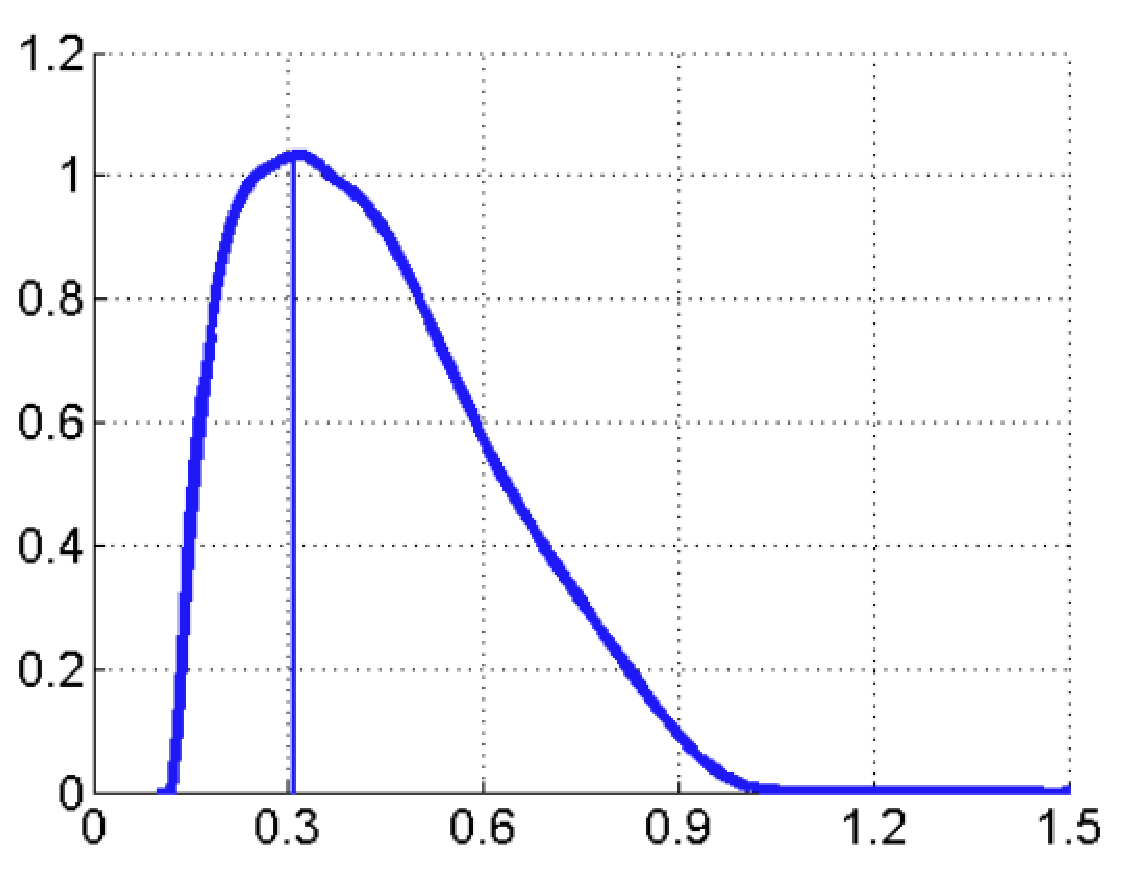
\includegraphics[width=0.35\textwidth]{figures/ch_free_energy/experimental_mututal_inf_chehreghani2012}%
\\[.5cm]
\caption{Experimental results for the averaged log-posterior agreement
  of a clustering problem 
  \citep{morteza12}.}
\label{fig:experiments-capacity}
\end{figure}%

% \begin{figure}[htbp]
% \centering 
% \noindent\includegraphics[width=\textwidth]{\dir/kernel.tikz}
% \caption{Schematic posterior agreement kernel $\hat{k}_\beta(X',X'')$
%   associated with the two-instance scenario
%   of~Fig.~\ref{fig:two-instance} is maximized at $\beta = 2.8$.}%
% \label{fig:two-instance-capacity}%
% \end{figure}

\begin{definition}\label{def:free_log_posteriors}
Further, analogically to ASC
$($cf.~\eqref{eq:asc_mutual_information_formula_wo_expct}$)$ we give a definition of
\textit{empirical log-posterior agreement}:
\begin{align}
  \hat I_\beta(X', X'') &\coloneqq \log \hat{k}_\beta(\data', \data'') \notag \\
    &=  \log \sum_{c \in \C} p_\beta(c | \data') p_\beta(c | \data'')
\end{align}
\index{Empirical log-posterior agreement}
\nomenclature[F, 07n]{$\hat I_\beta(X', X'')$}{empirical log-posterior agreement\mynomdef{def:free_log_posteriors}}%
and the \textit{expected log-posterior agreement}
$($cf.~\eqref{eq:asc_mutual_information_formula}$)$ as
\begin{align}
  I_\beta \equiv \mathrm{eLPA}_\beta &\coloneqq \Expct \hat I_\beta(X', X'') \notag \\ 
    &= \Expct \log \hat{k}_\beta(\data', \data'') \notag \\
    &= \Expct \log \sum_{c \in \C} p_\beta(c | \data') p_\beta(c
  | \data'').
\end{align}
\index{Expected log-posterior agreement}
\index{eLPA|see{Expected log-posterior agreement}}
\nomenclature[F, 07p]{$I_\beta$}{expected log-posterior agreement}%
\nomenclature[F, 07r]{$\mathrm{eLPA}_\beta$}{expected log-posterior agreement}%
\end{definition}

Finally, in full analogy with the original ASC (Chapter~\ref{ch:gen_appch}) we
introduce \textit{approximation capacity} (see Definition~\ref{def:asc_score})
which quantitatively measures the maximum of expected log-posterior agreement
(cf.~\eqref{eq:gibbs_realaxation}):
\begin{definition}\label{def:gencapacity}
The \textbf{approximation capacity} $I$ of a cost function $R(c,X)$
is defined as
\begin{align}\label{eq:gencapacity}
  I 
    &\coloneqq \sup_\beta \Expct_{X', X''} 
      \log |\C| \sum_{c \in \C} p_\beta(c | \data') p_\beta(c | \data'') \notag \\
    &\coloneqq \sup_\beta \Expct_{\data', \data''} \log\bigl(|\C|\;
    \hat{k}_\beta(\data', \data'') \bigr)\,.
\end{align}
\end{definition}
\index{Approximation capacity}

The optimal $\beta^*$ is thus, according
to Chapter~\ref{ch:gen_appch}, obtained through maximizing the eLPA:
\begin{equation}
  \beta^* \coloneqq \arg \max_\beta \Expct_{\data', \data''} \log\bigl(|\C|\;
      \hat{k}_\beta(\data', \data'') \bigr).
\end{equation} 
\nomenclature[F, 07u]{$\beta^*$}{optimal inverse temperature}%
The search for an optimal $\beta$ can also be interpreted as a selection of a
randomized algorithm that samples solution from a Gibbs posterior with the
respective $\beta$-controlled ``width''. In a toy example presented in
Figure~\ref{fig:two-instance-capacity} the posterior kernel is shown for
different values of $\beta$. We see that it has a clear maximum w.r.t. the
temperature, and this is always the case. In fact, this is also confirmed by
recent experimental results from~\citep{morteza12} shown in
Figure~\ref{fig:experiments-capacity}. In this chapter, in
Theorem~\ref{thm:gen_capacity_lqap_smbp} we provide theoretical justification
for such behavior by considering in details two optimization problems, namely
sparse Minimum Bisection Problem (sMBP) and Lawler's Quadratic Assignment
Problem (QAP).

\paragraph{Computing Free Energy Density}

In order to estimate the posterior kernel ~\eqref{eq:simker} we need to evaluate
$\Expct \log Z(\beta,\data')$, $\Expct \log Z(\beta, \data'')$  as well as
$\Expct \log \sum_{c\in \C} \exp\bigl(-\beta (R(c,\data') + R(c,\data''))\bigr)$, i.e.
the expected log-partition functions.  For a large $n$ this
task represents a computational bottleneck and is known to pose a notoriously difficult
mathematical challenge (see \cite{talagrand03}). We address this issue in our
work and provide new solutions and novel lower bounding techniques. More
precisely, 
%we will be interested in a version (note unsignificant difference
%from the conventional definition) of
we compute the \textit{Helmholtz free energy} density defined
in~\eqref{eq:free_energy_def}.
\begin{definition}
  The free energy density (or rate) of a set of solutions (configurations) $\C$ is
  defined as
  \begin{equation}
  \label{eq:free_energy_def}
    \frenergy(\beta) = -\Expct_X[\log Z( \beta, X)] / \log |\C| \;.
  \end{equation}
  \index{Configuration}
  \index{Free energy}
  \index{Free energy!Denisity}
  \index{Free energy!Rate}
  \index{Helmholtz free energy}
\end{definition}
\myremark Note the differences with the original definition
(Definition~\ref{def:background_free_energy}): first, we drop the $1/\beta$
scaling for convenience here; second, we use a scaling by $\log |\C|$, as we
refer to free energy \textit{density}. It is important that both scalings are
used for technical convenience and to ensure the existance of thermodynamic
limits ($n \to \infty$), therefore, we will mostly utilize the term ``free
energy'' without the word ``density''.



%\begin{figure}
  %\centering
  %\includegraphics[width=.5\textwidth]{figures/ch_free_energy/solution_set_illustration}
  %\caption{Schematic illustration of the objects set $\S_n$, feasible solutions
    %set $\C_n$, cost function $R(c,X)$ and related
    %notions.}
  %\label{fig:solution_set_illustration}
%\end{figure}

% In summary, computing the information content and adjusting the
% parameter $\beta$ for optimization problems requires to
% estimate the expectation of the logarithm of the partition function:
% $\Expct[\log Z(\beta, X)]$. 

It is known~\citep{Bovier2002FreeEnergyFluct,talagrand03}, that obtaining
asymptotic bounds for this quantity is a difficult mathematical problem. In
this chapter we tackle it for some special cases.

\subsection{Contributions and Outline of the Chapter}
\label{sec:free_energy_contribs}

As contributions of this chapter, we 
\begin{itemize}
  \item perform a mathematically rigorous asymptotic analysis of the free energy for 
  two optimization problems (i.e., sparse MBP and Lawler QAP described below in
  detail) for a high-temperature regime, proving matching upper and lower
  bounds. For both, we introduce novel methods of proving them. We shall find
  phase transitions which are equivalent to the discontinuities of REM and
  high-temperature SK~\citep{derrida81,Aizenman1987};
  \index{High-temperature regime}
  \index{Phase transition}
  \index{Free energy!Phase transition}
  \index{Free energy!Matching bounds}
  \item perform a rigorous asymptotic computation of \textit{expected log-posterior
  agreement (eLPA)}~--- a Gibbs relaxation of the ASC score. Original and Gibbs
  ASC scores were introduced in earlier chapters, cf.
  ~\eqref{eq:asc_best_gamma},~\eqref{eq:asc_mutual_information_formula} and
  \eqref{eq:gibbs_similarity_maximization_objective};
  \item we interpret the semantics of eLPA in a new way, supporting the ideas from
  Chapter~\ref{ch:gen_appch} and (indirectly) Chapter~\ref{ch:mst};
  \item we carry out experiments which give a firm ground for a conjecture about
  a form of the free energy in a general (i.e. not constrained to sMBP or Lawler
  QAP) problem cases. Surprisingly, this conjecture turns into proven asymptotics
  for cases of sMBP and Lawler QAP.
\end{itemize}

The chapter is organized as follows. First, an overview on the related work is
given in Section~\ref{sec:free_related_work}. Formal definitions and main result
theorems are stated in Section~\ref{sec:free_main_results}: in
Section~\ref{sec:free_opt_problem_under_consideration} the sMBP and Lawler QAP
optimization problems are described, while in
Section~\ref{sec:free_main_results_statements} (namely,
Theorems~\ref{thm:sparse_mbp_tight_bound}, \ref{thm:lawler_qap_tight_bound} and
\ref{thm:gen_capacity_lqap_smbp}) main results about them are provided. Proofs
of the main results can be found
in~Sections~\ref{sec:free_smbp_lowerbound_proof}
and~\ref{sec:free_lqap_lowerbound_proof}. In
Section~\ref{sec:free_experimental_mainresults}, an important intermediary
discussion is made. Further, in Section~\ref{sec:free_energy_in_general_case} we
perform an experimental evaluation of a more general case of non-sparse MBP, and
conjecture a surprisingly good ad-hoc formula for a free energy. In
Section~\ref{sec:free_free_energy:conclusion}, we discuss our results.

\section{Background and Related Work Overview}
\label{sec:free_related_work}

Combinatorial optimization arises in many real world settings and
these problems are often notoriously difficult to solve due to data
dependent noise in the parameters defining such instances.  Algorithms
that minimize these noisy instances or approximate their global
minimum return a solution that is a random variable due to input
randomness and that is most often highly unstable. Therefore, we 
ask the very reasonable questions: What is the distribution of the
output returned by the algorithm? Can we stabilize such an output
distribution by regularizing the algorithm?

Algorithm design in noise affected real world settings requires both
statistical as well as computational considerations: first, we have to
ensure that outputs of algorithms are typical in a statistical sense,
i.e., they have to occur with high probability. Second, such typical
outputs have to be computable in an efficient way with efficient
resources. 
%%% JB: The next comment can be removed. 
% The reader should notice that statistical requirements
% dominate computational ones in an epistemological sense: A
% computational result has to be rejected if it is atypical since it
% lacks predictive power. Computationally, we might require
% significantly different algorithmic resources (time and space) to
% calculate typical solutions for typical inputs.
%%% up to here.

Due to the statistical nature of inference, we have to efficiently compute
posterior distributions of solutions given input data. Open theoretical issues
emerge for this strategy, e.g., analytical computation of macroscopic properties
like entropy, expected log-partition function or expected
costs~\citep{moor85qap,talagrand03}. The expected log-partition function known
also as the \textit{free energy}, appeared in the context of combinatorial
optimization since the mid 80's; see e.g., the work by \citet{mezard84tsp}, who
explored the free energy properties of the traveling salesman problem.  An
intriguing property of free energy is the emergence of discontinuities of
certain order when changing the concentration of the posterior distribution.
Such abrupt changes of macroscopic properties, also known as \textit{phase
transitions}, are characteristic features of various large systems and have been
generating an uninterrupted interest in theory of discrete structures for a long
time~\citep[see][]{cohen88, LUCZAK1994}.
\index{Phase transition}

Free energy found also applications in theoretical computer science as discussed
in the previous section. We introduced a robustness score function called the
\textit{expected log-posterior agreement} (eLPA) for measuring ``goodness'' of
robust solutions. It is tightly connected to computing free energies, as wee
noted above. Furthermore, estimating the free energy for combinatorial
optimization problems allows us to justify theoretically some experimental
results obtained for these problems.

For the sake of completeness we should note here that the same, if not more
intensive, excitement has been generated for finding \textit{theoretical} laws
that govern the behavior of macroscopic thermodynamic properties in statistical
physics of large disordered particle systems.  Many interesting models of such
large systems were introduced relatively early,~e.g. the
\textit{Sherrington-Kirkpatrick (SK) spin glass model}~\citep[see][]{sk75spin}.
It took, however, some time and effort to develop rigorous techniques for
solving them. For example, \citet{derrida81} introduced a very simple, but
exactly solvable model called \textit{random energy model (REM)} as the limit of
SK models family. Later, \citet{Aizenman1987} published an exact solution in the
high-temperature phase for SK model. The general question about the exact free
energy behavior became increasingly motivating: it triggered a new wave of
latest research \citep[see][]{Bovier2002FreeEnergyFluct, talagrand03}. The
reader should also note that many interesting heuristic tools were developed in
the context of statistical physics over the last several decades, such as the
replica method~\citep{Parisi2009replica}, the cavity
method~\citep{Mezard2003Cavity} and mean-field approximation schemes with belief
propagation algorithms.
\index{Random Energy Model}
\index{Sherrington-Kirkpatrick model}
\index{SK model|see{Sherrington-Kirkpatrick model}}
\index{Spin glass}

\section{Main Results}
\label{sec:free_main_results}

In this chapter we focus on two optimization problems, namely the sparse Minimum
Bisection Problem (sMBP) and the Lawler Quadratic Assignment Problem (LQAP).
Formal definitions are given below. However, we should add that many of our
results hold for a larger class of optimization problems as long as $\log
m=o(N)$~\citep[see][]{ws95optimization}.  In the rest of the chapter we will
utilize the temperature rescaling $\beta = \hat \beta \sqrt{\log m/N}$ with
$\hat \beta = \mathcal{O}(1)$ which together with $\log m = o(N)$ explains $\beta
\to 0$ limit. This rescaling was justified in~\citep{aofa2014}.

For these two problems  we shall provide  
 tight asymptotics for the free energy~\eqref{eq:free_energy_def}, and
compute asymptotically the log-posterior agreement as well as $\hat \beta^*$
that maximizes the posterior kernel.

\subsection{Minimum Bisection and Quadratic Assignment Optimization Problems}
\label{sec:free_opt_problem_under_consideration}

This section introduces the combinatorial optimization problems that will be used to
describe our findings. These problems fall into the $\log m = o(N)$ class
specified in Sec.~\ref{sec:free_setting_notation} and cover a wide range of
practical applications in signal processing and neural information processing.

%%%%%%%%%%%%%%%%%%%%%%%%%%%%%%%%%%%%%%%%%%%%%%%%%%%%%%%%%%%%%%%%%%%%%%%%%%%%%%%%%%%%%%%%%%%%%%
\paragraph{Minimum bisection problem (MBP)} 
\label{sec:free_mbp-problem}
Consider a complete undirected weighted graph $G=(V,E,X)$ of $n$ vertices, where
$n$ is an even number. The input data instance $X$ is represented by (random) weights
$(W_i)_{i\in E}$ of the graph edges.
A \textit{bisection} is a balanced partition $c=(U_1,U_2)$ of the vertices in two
disjoint sets: $U_1, U_2\subset V$, $U_1 \sqcup U_2 = V$,
$|U_1|=|U_2|=\frac{n}{2}$. 
Now $\S_n = E$ and $\C_n$ is the set of all bisections of graph
$G$, while $\mathcal{S}_n(c)$ is the set of all edges cut by the bisection $c$.
The cost of a bisection $c$ is the sum of the weights of all cut edges
\begin{equation}
  R(c, X) = \sum_{i\in\mathcal{S}_n(c)} W_i.
\end{equation}
\index{Minimum Bisection Problem}
\index{MBP|see{Minimum Bisection Problem}}
\nomenclature[F, 09a]{$G=(V,E,X)$}{random graph instance\nomnorefeq}%
\nomenclature[F, 09c]{$(W_i)_{i\in E}$}{edge weights\nomnorefeq}%
\nomenclature[F, 09e]{$(U_1,U_2)$}{bisection\nomnorefeq}%


The minimum bisection problem finds the bisection of a graph
with minimum cost. A simple calculation (we omit here $1/2$ constant
for the sake of brevity) shows that $|\C_n| = m = \binom{n}{n/2}$ and
$|\mathcal{S}_n(c)| = N =
\frac{n^2}{4}$, and that
\begin{equation}
  \log m = \log \binom{n}{n/2} \sim \log \biggl( 2^n \sqrt{\frac{2}{\pi n}}\biggr) =
    n\log 2 - \frac{1}{2} \log n + \mathcal{O}(1),
\end{equation}
which shows that the minimum bisection problem belongs to the class of stochastic
optimization problems discussed in this work (i.e., $\log m = o(N)$).
\nomenclature[A, 03a]{$\binom{n}{k}$}{binomial coefficient}%
\nomenclature[A, 03c]{$\mathcal{O}(\cdot)$}{upper-bounded (constant factor)\nomnorefeqpage}%
\nomenclature[A, 03d]{$o(\cdot)$}{infinitely smaller\nomnorefeqpage}%
\nomenclature[A, 03f]{$\Theta(\cdot)$}{upper- and lower-bounded (constant factor)\nomnorefeqpage}%

\paragraph{Sparse minimum bisection problem (Sparse MBP, sMBP)}
\label{sec:free_sparse_mbp}
\begin{figure}[htbp]
  \centering
  \includegraphics[width=.7\linewidth]{figures/ch_free_energy/smbp_illustration}
  \\[.5cm]
  \caption{Illustration of the sparse Minimum Bisection Problem (sMBP) introduced
  in Section~\ref{sec:free_opt_problem_under_consideration}.}
  \label{fig:free_smbp_illustration}
\end{figure}

\index{Sparse Minimum Bisection Problem}
\index{Sparse MBP|see{Sparse Minimum Bisection Problem}}
\index{sMBP|see{Sparse Minimum Bisection Problem}}
We actually will focus on the \textit{sparse} Minimum Bisection Problem in which
the disjoint subsets are of the size $|U_1|=|U_2|\equiv d$ where $d$ grows
faster than $\log n$ and slower than $n$ (which we write $\log n \ll d \ll n$).
Thus, $N = d^2$ and the following holds
\begin{equation}
  \log m = \log \binom{n}{d} \binom{n-d}{d} = 
    \log \frac{n!}{d! (n-2d)!} \sim 2d \log n .
\end{equation}
Thus the problem falls into the class $\log m = o(N)$ since we assume $\log n \ll d$.
\nomenclature[F, 09g]{$d$}{half-bisection size\nomnorefeq}%

%%%%%%%%%%%%%%%%%%%%%%%%%%%%%%%%%%%%%%%%%%%%%%%%%%%%%%%%%%%%%%%%%%%%%%%%%%%%%%%%%%%%%%%%%%%%%%
\paragraph{Quadratic Assignment Problem (QAP)}
\label{sec:free_qap_definition}
We consider two $n\times n$ real-, positive-valued matrices, namely the weight
matrix $V$ and the distance matrix $H$.  The solution space $\C_n$ is the set of
the $n$-element permutations $\mathbf{S}_n$.  The cost function is then $R(\pi,
V, H) = \sum_{i,j=1}^n V_{ij}\cdot H_{\pi(i),\pi(j)}$ for $\pi\in \mathbf{S}_n$. 
In our terms, the object space is the set of products of entries
of $V$ and $H$ constrained by a relation on the indices: $ \S_n = \{ V_{ij}\cdot
H_{\pi(i),\pi(j)} \mid 1 \le i,j \le n; \pi
\in \mathbf{S}_n \}.$
In our notation, $N=|\mathcal{S}_n(\pi)|=n^2$ and $m=|\C_n|=n!$ and thus $\log m
\sim n \log n = o(N)$ is satisfied.
\index{Quadratic Assignment Problem}
\index{QAP|see{Quadratic Assignment Problem}}

\paragraph{Lawler Quadratic Assignment Problem (Lawler QAP)}
\label{sec:free_lawler}
\cite{lawler1963quadratic} introduced a generalization of the QAP
where the distance and weight matrices are replaced by a 4-dimensional matrix
$Q$ with i.i.d. values: $R(\pi, Q) = \sum_{i,j=1}^n Q_{i,j,\pi(i),\pi(j)}$ for
$\pi\in \mathbf{S}_n$. 
It is interesting to see that this generalization does not
change the combinatorial structure of the problem: a Lawler QAP can be built
from a normal QAP and thus falls into our class.
\index{Quadratic Assignment Problem}
\index{Lawler QAP|see{Lawler Quadratic Assignment Problem}}
\index{LQAP|see{Lawler Quadratic Assignment Problem}}

% \textbf{Remark.} Observe that from a stochastic point of view, if we now generate
% \emph{i.i.d.} values for the entries of $D$ (instead of generating
% \emph{i.i.d.} values for the entries of $V$ and $H$), most of the
% dependencies disappear. In fact, the dependencies boil down to solutions
% sharing entries of matrix $D$: two solutions $\pi$ and $\pi'$ are
% dependent if and only if there exists an index $i$ such that $\pi(i)=\pi'(i)$.
% Thus the dependency is reduced.

%%%%%%%%%%%%%%%%%%%%%%%%%%%%%%%%%%%%%%%%%%%%%%%%%%%%%%%%%%%%%%%%%%%%%%%%%%%%%%
%%%%%%%%%%%%%%%%%%%%%%%%%%%%%%%%%%%%%%%%%%%%%%%%%%%%%%%%%%%%%%%%%%%%%%%%%%%%%%

\subsection{Free Energy and its Phase
  Transition}
\label{sec:free_main_results_statements}

In order to give a full picture, before presenting our main results we 
first derive a tight upper bound on the free energy as discussed
in \citep{aofa2014}.  Interestingly, it shows
that there is a phase transition in the second-order term of the upper bound of
the free energy. Such a phase transition is a characteristic feature of various
large-scale systems~\citep[see][]{LUCZAK1994, talagrand03,
MM:AM:IPC2009}.

First, let us state our main assumptions that we use throughout the chapter.

\index{Common Theorem Setting}
\index{CTS|see{Common Theorem Setting}}
\begin{definition}[Common Theorem Setting]
\label{def:cts}
Consider a class of combinatorial optimization problems in which:
\begin{itemize}
\item[{\rm (A)}] the cardinality
$m$ of the set of feasible solutions and the size $N$ of every feasible
solution are related as $\log m=o(N)$, and we adopt the scaling
$\beta=\hb \sqrt{ \log m / N}$; 
\nomenclature[F, 11a]{$\hb$}{scaled inverse temperature\nomnorefeq}%
\item[{\rm (B)}]
weights $W_i$ are identically (not necessarily independently) distributed with
mean $\mu$ and variance $\sigma^2$ and that the moment-generating function
\index{Moment-generating function} of the negative centralized weights
$(-\bar{W}_i)$ is finite, i.e.~$\bar G(t) \equiv
\Expct[\exp(-t\bar{W}_i)]<\infty$ exists for some $t>0$;
\nomenclature[F, 03]{$\bar G(t)$}{moment-generating function\nomnorefeq}%
\nomenclature[F, 11c]{$\bar{W}_i$}{centralized weights\nomnorefeq}%
\item[{\rm (C)}] 
within a given solution $c$, the weights are mutually independent, i.e. for all
$c\in \C_n$, the set $\{W_i \mid i\in\mathcal{S}_n(c)\}$ is a set of mutually
independent variables.
\end{itemize}
\end{definition}

\begin{theorem}
\label{thm:general-upper-bound}
Under the common theorem setting of the current section the following holds:
\begin{equation}
  \lim_{n\to \infty} \frac{\E[\log Z(\beta, X)] +\hat \beta \mu \sqrt{N\log m}}{\log m}
  \leq
  \begin{cases}
    1+\frac{\hb^2\sigma^2}{2}, &\hb< \frac{\sqrt{2}}{\sigma},\\
    \hb \sigma \sqrt{2}, &\hb\ge \frac{\sqrt{2}}{ \sigma}.
  \end{cases}
\end{equation}
\end{theorem}

\nomenclature[F, 11aa]{$\tilde \beta$}{unit-free rescaled inverse temperature\nomnorefeq}% 
\myremark As it can be seen from the above theorem, a unit-free rescaling 
$\tilde \beta = \hat \beta \sigma$ could simplify the formulation. Further,
we use the initial rescaling for clarity.


\myremark The general upper bound proven  above
is unfortunately not tight. Consider the (non-sparse) minimum bisection
problem with $d=n/2$. Under the same general assumptions for the weights,
it can be shown that a tighter bound holds for $\hat{\beta} \leq
\frac{1}{\sqrt{\log 2}\sigma}$
\begin{equation}
\label{SK_th}
  \lim_{n\to \infty} \frac{\E[\log Z(\beta, X)] +\hat \beta \mu \sqrt{N\log m}}{\log m}
    \leq 1 + \frac{\hat{\beta}^2\sigma^2}{4}.
\end{equation}
We prove \eqref{SK_th} in Section~\ref{sec:free_sk}. \QEDA
\par
\medskip

\paragraph{Proof of Theorem~\ref{thm:general-upper-bound}} 
\index{Inequality!Jensen's}
\index{Jensen's inequality|see{Inequality}}
To get a flavor of bounding $\Expct[ \log Z]$ we first observe that  $\Expct[
\log Z] \leq \log \Expct[ Z]$ (by Jensen's inequality). We can evaluate 
$\Expct[Z]$ as follows:
\begin{align}
  \Expct[Z] &= \Expct\Bigl[\sum_{c\in \C} \exp(-\beta R(c))\Bigr] \notag \\
    &= \exp(-\beta N \mu) \Expct\Bigl[\sum_{c\in \C} \exp\bigl(-\beta
      (R(c)-N\mu)\bigr)\Bigr] \notag \\ 
    &=\exp(-\beta N \mu) m \bar G^N(\beta).
\end{align}
Thus
\begin{equation}
\label{spa1}
\log \Expct[Z]=-\beta N \mu+ \log m + N \log \bar G(\beta)
\end{equation}
since the set of random variables $W_i$ belonging to the same solution  
are mutually independent variables.
Throughout we write $\bar R(c)=R(c)-\Expct[R]=R(c) -N\mu$ for the 
centralized cost, and $\bar G(\beta)$ for the moment generating function of 
the negative centralized weight $\bar W=W - \mu$:
\begin{equation}
  \bar G(\beta) \coloneqq \Expct \exp(-\beta \bar W).
\end{equation}
\nomenclature[F, 11e]{$\bar R(c)$}{centralized cost\nomnorefeq}%

\index{Taylor series}
We can expand $\bar G(\beta)$ into the Taylor series around zero and obtain
\begin{equation}
\bar G(\beta)=1+\frac 12 \beta^2 \sigma^2 + \mathcal{O}(\beta^3).
\end{equation}
We find as long as $\beta\to 0$
\begin{align}
\label{e-EZ}
\log \Expct[Z]&= -\beta N \mu+ \log m +N\log \bar G(\beta) \notag \\
  &= -\beta N \mu+ \log m + N \log\Bigl(1+\frac 12 \beta^2 \sigma^2 + \mathcal{O}(\beta^3)\Bigr) \notag \\
  &= -\beta N \mu+ \log m +\frac 12 N \beta^2 \sigma^2(1+ \mathcal{O}(\beta)).
\end{align}
Now we apply the rescaling from the Common Theorem Setting
\begin{equation}
\label{spa2}
\beta=\hb \sqrt{\frac{\log m}{N}}
\end{equation}
for some constant $\hb$ leading to 
\begin{equation}
\label{spa3}
\frac{\log \Expct[Z]+\beta N \mu}{\log m}= 1+ \frac 12 \hb^2 \sigma^2 (1+\mathcal{O}(\beta)).
\end{equation}
In terms of $\Expct[\log Z]$ we find
\begin{equation}
\label{spa4}
\frac{\Expct[ \log Z] +\hb \mu \sqrt{N \log m}}{\log m} \leq
1+ \frac 12 \hb^2 \sigma^2 \biggl(1+\mathcal{O}\biggl(\sqrt{\frac{\log m}{N}}\biggr)\biggr).
\end{equation}

But there is a surprise! Let us denote
\begin{equation}
  \phi(\beta) = \Expct[\log Z] +\beta N \mu=: \Expct[\log \hat{Z}(\beta)]
\end{equation}
\nomenclature[F, 11g]{$\hat{Z}(\beta)$}{scaled partition function}%

where $\hat{Z}(\beta)=\sum_{c \in \C} \exp(\beta \bar{R}(c))$ with
$\bar{R}(c)=-\sum_{i \in \S(c)} \bar{W}_i$.  It is easy to observe
that
\begin{equation}
\beta \max_{c\in \C} \bar{R}(c) \leq \log \hat{Z}(\beta).
\end{equation}
Using the upper bound obtained in (\ref{spa4}) we  find
\begin{equation}
\label{spa5}
\frac{\Expct[\max_{c\in \C} \bar{R}(c)]}{\log m} \leq  \sqrt{\frac{N}{\log 
    m}} \left( {\hb}^{-1}+\frac 12 \hb \sigma^2 \right). 
\end{equation}
\index{Critical inverse temperature|see{Inverse temperature}}
\index{Inverse temperature!Critical}
Choosing a critical inverse temperature $\hb_c=\sqrt{2}/\sigma$ 
that minimizes the right-hand side of (\ref{spa5}) we arrive at
\begin{equation}
  \Expct[\max_{c\in \C} \bar{R}(c)] \leq \sqrt{2\sigma^2 N \log m} 
% =\hb \sigma \sqrt{2} \log m
\end{equation}
Now proceeding as in \citet[Proposition~1.1.3]{talagrand03}
we obtain
\begin{equation}
\phi'(\beta) \leq \Expct[\max_{c\in \C} \bar{R}(c)].
\end{equation}
But for $\beta > \beta_c \coloneqq \hb_c\sqrt{\log m / N}$,
\begin{equation}
    \phi(\beta)
    \leq \phi(\beta_c) + \phi'(\beta_c)(\beta - \beta_c),
\end{equation}
\nomenclature[F, 11j]{$\beta_c$}{critical inverse temperature}%
since $\phi(\beta)$ is known to be convex.  Applying the
upper bound for $\phi'(\beta)$ yields 
\begin{equation}\label{second_upper}
\Expct[\log \hat Z] \leq \hb \sigma \sqrt{2} \log m
\end{equation}
and the upper bound for the second $\hat\beta$ region is obtained.
Observe that in this region the growth is linear with respect to $\hb$. 

In summary, Theorem~\ref{thm:general-upper-bound} is proven. \QEDA

%\subsection{Matching Lower Bound for Sparse MBP}
%\label{sec:free_smbp_mainresults}

For some combinatorial optimization problems, the asymptotic upper bound of
Theorem~\ref{thm:general-upper-bound} turns out to be tight. Below we present
our two main results which give the asymptotically matching lower bounds for the
Sparse MBP and Lawler QAP. For the Sparse MBP we develop a novel approach of
proving it since the techniques  proposed by~\citet[][Chapter 1]{talagrand03}
seem not to work.%We formulate the matching lower bound for sMBP first.
%The conditions are supposed to comply with
%the common setting given in the beginning of this section.

% The latter lower bound uses a technique suggested by
% Talagrand while for the former lower bound we invented a new approach since the
% Talgarad's method seems not to be working.

\begin{theorem}\label{thm:sparse_mbp_tight_bound}
  Consider the Sparse MBP complying with the Common Theorem Setting whose edge weights
  have mean $\mu$ and variance $\sigma^2$. Then the following holds:
\begin{equation}\label{eq:sparse_mbp_tight_bound}
\lim_{n\to \infty} \frac{\E[\log Z(\beta, X)] +\hat \beta \mu \sqrt{N\log m}}{\log m} =
\left\{ \begin{array}{ll}
1+\frac{\hat \beta^2\sigma^2}{2}, &
\hat \beta< \frac{\sqrt{2}}{\sigma},\\
\hat \beta \sigma \sqrt{2}, & \hat \beta \ge \frac{\sqrt{2}}{\sigma}
\end{array}
\right.
\end{equation}
provided $\log \ll d \ll n^{2/7}/\sqrt{\log n}$.
\end{theorem}

Let us now consider the Lawer QAP. In this case, we apply a slightly modified
approach developed in~\citeauthor{talagrand03}. However, we should point out that
Lawer's QAP has some dependency that were not present in Derrida's model
for which Talagrand proposed his method. 


%\subsection{Matching Lower Bound for Lawler QAP}
%\label{sec:free_lqap_mainresults}

\begin{theorem}\label{thm:lawler_qap_tight_bound}
  Consider Lawler QAP complying with Common Theorem Setting, whose matrix
  entries have mean $\mu$ and variance $\sigma^2$. Then the following holds:
\begin{equation}\label{eq:lawler_qap_tight_bound}
\lim_{n\to \infty} \frac{\E[\log Z(\beta, X)] +\hat \beta \mu \sqrt{N\log m}}{\log m} =
\left\{ \begin{array}{ll}
1+\frac{\hat \beta^2\sigma^2}{2}, &
\hat \beta< \frac{\sqrt{2}}{\sigma},\\
\hat \beta \sigma \sqrt{2}, & \hat \beta \ge \frac{\sqrt{2}}{\sigma}.
\end{array}
\right.
\end{equation}
\end{theorem}

\myremark Proofs of both theorems will be given in separate Sections~\ref{sec:free_smbp_lowerbound_proof}
and~\ref{sec:free_lqap_lowerbound_proof} due to their length.

\subsection{Expected Log-Posterior Agreement Asymptotics}

The above two theorems allow to operate (in a theoretically justified way) with
the free energy, which, as we stated in the introduction, is
a well-known \textit{mathematical} (or \textit{statistical mechanical}) problem.
However, we would like to bring the connection to a more applied field as well:
namely, to robust sampling. By that we refer once more to the definitions of
log-posterior agreement (eLPA) and generalization capacity
(see~\eqref{eq:simker} and~\eqref{eq:gencapacity}). We recall the intuition
behind these two notions: they serve the purpose of selecting the ``best''
temperature ($\beta$) for a Gibbs distribution over the solutions to a
combinatorial problem.

%What is the connection between these notions and
The matching lower bounds for sMBP and Lawler QAP given above in 
Theorems~\ref{thm:sparse_mbp_tight_bound}
and~\ref{thm:lawler_qap_tight_bound} 
allow us to present theoretical justification for the behavior of the
posterior agreement kernel as shown in Figure~\ref{fig:experiments-capacity}.
To see that, we observe that
\begin{align}
\label{eq:log_posterior_rewritten}
  \Expct_{X', X''} \log &\sum_{c \in \C} p_\beta(c|X') p_\beta(c|X'') \\ \notag
    &= \Expct_{X',X''} \log \sum_{c \in C} \frac{\exp(-\beta (R(c, X') + R(c,X'')))}{Z(\beta, X') Z(\beta, X'')} \\
    &= \Expct_{X',X''} \log Z(\beta, X', X'') - \Expct_{X'} \log Z(\beta, X') 
      - \Expct_{X''} \log Z(\beta, X''),
\end{align}
where $Z(\beta, X',X'')$ can naturally be defined as a ``partition function''.
\begin{equation}
  Z(\beta, X', X'') \coloneqq \sum_{c \in C} \exp(-\beta (R(c, X') + R(c,X''))).
\end{equation}
Eventually this allows us to use the above theorems to compute all the three
terms of~\eqref{eq:log_posterior_rewritten}.

To make the final step, we first need to formalize how exactly $X'$ and $X''$ are
obtained: let us assume that the two instances $X'$ and $X''$ are both
represented by two sets of weights $X' = \{W_i'\}$ and $X'' =
\{W_i''\}$ through adding two ``noise'' instances $\delta X' = \{\delta W_i'\}$
and $\delta X'' = \{\delta W_i''\}$ to the same ``signal'' instance
$X = \{W_i\}$ all the mentioned sets being of the same size $|\S|$:
\begin{equation}
  W_i' = W_i + \delta W_i', \quad W_i'' = W_i + \delta W_i'' 
    \quad \text{for} \quad i \in \S.
\end{equation}
We also require that the signal and noise weights have certain means and
variances:
\begin{align}
  \Expct [W_i] &= \mu &  \Var [W_i] &= \sigma^2 \\ 
    \Expct [\delta W_i'] &= \Expct [\delta W_i''] = 0 & 
    \Var [\delta W_i'] &= \Var [\delta W_i''] = \tilde \sigma^2.
\end{align}
We define the \textit{noise-to-signal ratio} as $\gamma=\tilde \sigma/\sigma$.
Applying Theorems~\ref{thm:sparse_mbp_tight_bound}
and~\ref{thm:lawler_qap_tight_bound} we are led to the following result for
the posterior agreement kernel (the consequences of this result will be discussed later in
Section~\ref{sec:free_experimental_mainresults}).
\index{Noise-to-signal ratio}
\nomenclature[F, 11n]{$\gamma$}{noise-to-signal ratio}%

\begin{theorem}\label{thm:gen_capacity_lqap_smbp}
Consider Sparse MBP or Lawler QAP complying with the Common Theorem Setting. Let
set $X$ be ``signal'' weights with mean ${\mu}$ and variance ${\sigma}^2$ and
two sets $\delta X'$, $\delta X''$ be ``noise'' with mean $0$, and variance
$\tilde{\sigma}^2$, all the sets of the same size. Let $X'=X+\delta X'$ and
$X''=X+\delta X''$ (elementwise sum) be the two problem instances. Let 
$\gamma \coloneqq \tilde\sigma/\sigma$ be noise-to-signal ratio. Then the expectation 
of the log-posterior agreement~\eqref{eq:simker} satisfies
\begin{equation}
  \lim_{n\to \infty} 
  \frac{\Expct_{X,\delta X',\delta X''} \log\bigl(|\C|\;
      \hat{k}_\beta(\data', \data'') \bigr)}
  {\log m}
    = \eta(\hb),
\end{equation}
\index{Noise-to-signal ratio}
where
\begin{equation}\label{eq:gc_three_phases}
  \eta(\hb) =
  \begin{cases}
    (\hb{\sigma})^2, & \hb {\sigma} < \frac{\sqrt{2}}{\sqrt{4+2\gamma^2}} \\
    \hb{\sigma}\sqrt{2}\sqrt{4+2\gamma^2} - (\hb{\sigma})^2(1+\gamma^2) - 1, 
      & \frac{\sqrt{2}}{\sqrt{4+2\gamma^2}} 
        \leq \hb{\sigma}
        < \frac{\sqrt{2}}{\sqrt{1+\gamma^2}} \\
    \hb{\sigma}\sqrt{2}
      \bigl(\sqrt{4+2\gamma^2} 
        - 2\sqrt{1+\gamma^2}\bigr) + 1, 
      & \frac{\sqrt{2}}{\sqrt{1+\gamma^2}} \leq \hb{\sigma}
  \end{cases}
\end{equation}
In particular, the expected log-posterior agreement is maximized at the eLPA-optimal
inverse temperature:
\begin{equation}\label{eq:elpa_optimal_temperature}
  \hat{\beta}^* \equiv \hat{\beta}^*_{\mathrm{eLPA}} = \frac{\sqrt{2+\gamma^2}}{\sigma(1+\gamma^2)}.
\end{equation}
\index{Optimal inverse temperature|see{Inverse temperature}}
\index{Inverse temperature!Optimal}
\nomenclature[F, 07ua]{$\hat{\beta}^*_{\mathrm{eLPA}}$}{eLPA-optimal scaled inverse temperature}%
% $\hat{\beta}^* = \frac{\sqrt{4\tilde{\sigma}^2+2\sigma^2}}
% {\sqrt{2}(\tilde{\sigma}^2+\sigma^2)}$.
\end{theorem}

\subsection{Proof of Theorem~\ref{thm:sparse_mbp_tight_bound}: Matching Lower Bound 
for sMBP}
\label{sec:free_smbp_lowerbound_proof}

In this section we present a proof of the matching lower bound for Sparse
MBP. The proof technique that we propose here is novel to the best of our
knowledge and was also used in \citep[see][]{magner2015protein,magner2016isit}.

The proof is broken into several lemmas. Let us start with defining $D$ as
elementwise overlap between two solutions (i.e.~number of shared \textit{edges})
sampled \textit{uniformly at random}. We will refer to this uniform distribution
as $\D$.
\nomenclature[F, 19a]{$D$}{random solution overlap\nomnorefeq}%
\nomenclature[F, 19b]{$\mathcal{D}$}{uniform distribution over solutions\nomnorefeq}%
\index{Elementwise solution overlap}
%\textit{edge-non-overlapping} and
%\textit{vertex-non-overlapping} pairs solutions.

\begin{lemma}\label{lem:vertex_non_overlap}
The following holds
  \begin{equation}
    \frac{\#\{\text{vertex-non-overlapping}\}}{m^2} = 1 - \Theta(d^2/n).
  \end{equation}
  \nomenclature[A, 00e]{$\vert\{\ldots\}\vert$, $\#\{\ldots\}$}{cardinality of a set\nomnorefeqpage}%
\end{lemma}
\parsec
\paragraph{Proof}
Observe that
\begin{align}\label{eq:vertex_non_overlap}
  \frac{\#\{\text{vertex-non-overlapping}\}}{m^2} 
    &= \frac{\binom{n}{d} \binom{n-d}{d} \binom{n-2d}{d} \binom{n-3d}{d}}%
      {\binom{n}{d}^2 \binom{n-d}{d}^2} \notag \\
    &= \frac{\binom{n-2d}{d} \binom{n-3d}{d}}%
      {\binom{n}{d} \binom{n-d}{d}}.
\end{align}
We now use Stirling's approximation, for any integer $c$ to find
\begin{align}
  \binom{n - cd}{d} &\le \frac{(n - cd)^d}{d!} \notag \\
    &= \frac{n^d ( 1 - cd/n)^d}{d!} \notag \\
    &\sim \frac{n^d (1 - cd^2/n)}{d!}.
\end{align}
Similarly,
\begin{align}
  \binom{n - cd}{d} &\ge \frac{(n - (c+1)d)^d}{d!} \notag \\
    &= \frac{n^d ( 1 - (c+1)d/n)^d}{d!} \notag \\
    &\sim \frac{n^d (1 - (c+1)d^2/n)}{d!}.
\end{align}
Applying these bounds we find
\begin{equation}
  \frac{\#\{\text{vertex-non-overlapping}\}}{m^2} 
    \le \frac{(1 - 2d^2/n) (1 - 3d^2/n)}{(1 - d^2/n) (1 - 2d^2/n)}
    \sim 1 - 2d^2/n
\end{equation}
and
\begin{equation}
  \frac{\#\{\text{vertex-non-overlapping}\}}{m^2} 
    \ge \frac{(1 - 3d^2/n) (1 - 4d^2/n)}{(1 - d^2/n)}
    \sim 1 - 6d^2/n.
\end{equation}
This completes the proof.
\QEDA

\begin{lemma} \label{lem:prob_d_zero_equivalence}
  The following holds:
  \begin{equation}
  \Prob_\D(D = 0) \sim \frac{\#\{\text{vertex-non-overlapping}\}}{m^2}
  \end{equation}
\end{lemma}
\parsec
\paragraph{Proof}
  \begin{align}
    \Prob_\D(D = 0) &= \frac{\#\{\text{vertex-non-overlapping}\}}{m^2} \\ \notag  
        &+ \frac{\#\{\text{edge-non-overlapping}\mid\text{vertex-overlapping}\}}{m^2}.
  \end{align}
  Since the following inclusion holds:
  \begin{equation}
    \{\text{edge-non-overlapping}|\text{vertex-overlapping}\} 
      \subseteq \{\text{vertex-overlapping}\},
  \end{equation}
  we can conclude that
  \begin{align}
    \frac{\#\{\text{edge-non-overlapping}\mid\text{vertex-overlapping}\}}{m^2} 
      &\le \frac{\{\text{vertex-overlapping}\}}{m^2} \notag \\
        = \frac{m^2 - \{\text{vertex-non-overlapping}\}}{m^2} 
      &= 1 - 1 + \Theta(d^2/n) \notag \\
      &= o(1),
  \end{align}
where the last equation comes from~Lemma~\ref{lem:vertex_non_overlap} and
  $d =o(n)$.
  Hence, the the following holds:
  \begin{align}
    \frac{\Prob_\D(D = 0)}{\#\{\text{vertex-non-overlapping}\}/m^2} 
      &= 1 \\ \notag 
      &\!\!\!\!\!\!\!\!\!\!\!\!\!\!\!\!\!\!\!\!\!\!\!\!\!\!\!\!\!\!+ 
          \frac{\#\{\text{edge-non-overlapping}\mid\text{vertex-overlapping}\}/m^2}%
        {\#\{\text{vertex-non-overlapping}\}/m^2} \notag \\
      &= 1 + \frac{o(1)}{1 + o(1)} \notag \\
      &= 1 + o(1),
  \end{align}
  which proves the lemma.
\QEDA
\par
\medskip

These lemmas allow us to estimate the expected value of $D$. 

\begin{lemma}\label{lem:expct_d_asymptotics}
  The following holds:
  \begin{equation}
    \Expct_\D D = \mathcal{O}(d^4 / n).
  \end{equation}
\end{lemma}
\parsec
\paragraph{Proof} 
To compute $\Expct_\D D$,  observe
\begin{align}
  \Expct_D D &= 0 \cdot \Prob_\D(D = 0) + \sum_{k=1}^N k \cdot \Prob_\D(D = k) \notag \\
    &\le N \sum_{k=1}^N \Prob_\D(D = k) \notag \\
    &= d^2 \cdot \Prob_\D(D \ne 0) = d^2 \bigl(1 - \Prob_\D(D = 0)\bigr) 
      \sim \Theta(d^4/n),
\end{align}
where the last asymptotic equivalence follows from
Lemmas~\ref{lem:vertex_non_overlap} and~\ref{lem:prob_d_zero_equivalence}. 
The less-than-equal sign turns $\Theta$ into $\mathcal{O}$. The lemma is proven.
\QEDA
\par
\medskip

We also state the lemma which establishes the behavior of $\Var Z$.

\begin{lemma}% [{\citealp[Lemma 1]{aofa2014}}]
\label{lemma:variance_z}
For any $\beta>0$ we have
\begin{equation}
\label{eq-var}
\Var Z = (\Expct Z)^2 \Bigl( \Expct_\D 
    \Bigl( \frac{G(2\beta)}{G^2(\beta)} \Bigr)^D - 1 \Bigr)
\end{equation}
where $D$ is a  random variable denoting the size of the elementwise overlap for
two solutions $c,c'\in \C$, chosen uniformly at random (this uniformness is 
referred by $\mathcal{D}$). Here, $G(\beta)$ is the
moment generating function of the negative weights $(-W_i)$. 
\end{lemma}
\parsec
\paragraph{Proof}
Let
\begin{equation}
Z(\beta) = \exp(-\beta N \mu) \hat{Z}(\beta),
\end{equation}
where, as previously, $\hat{Z}(\beta)=\sum_{c \in \C} \exp(\beta \bar{R}(c))$
with $\bar{R}(c)=-\sum_{i \in \S(c)} \bar{W}_i$.
To compute $\Var \widehat Z$, we proceed as follows
\begin{align}
  \Expct \widehat{Z}^2 &= \Expct \Bigl[ \sum_{c \in \C} \exp(\beta \bar{R}(c)) 
    \cdot \sum_{c' \in C} \exp(\beta \bar{R}(c')) \Bigr] \\ \notag
  &= \sum_{c, c' \in \C} \Expct  \exp\Bigl( -\beta \Bigl( \sum_{i \in \S(c)} 
    \bar{W}_i + \sum_{j \in \S(c')} \bar{W}_j \Bigr) \Bigr).
\end{align}
Now define the elementwise overlap between the solutions $c$ and $c'$ as
$\S_{\mathrm{ovr}}(c,c') \coloneqq \S(c)
\cap \S(c')$, and its cardinality $d = d(c,c') \coloneqq |\S(c, c')|$. 
We also define the symmetric difference $\bar \S_{\mathrm{ovr}}(c,c') \coloneqq \S(c)
\triangle \S(c')$ and continue the chain of equalities:
\begin{equation}
\Expct \widehat{Z}^2 
  = \sum_{c, c' \in \C} \Expct \exp\Bigl( 
    -\beta \Bigl( 
      2\sum_{i \in \S_{\mathrm{ovr}}(c,c')} \bar{W}_i 
      + \sum_{j \in \bar\S_{\mathrm{ovr}}(c,c')} \bar{W}_j 
    \Bigr)  
  \Bigr).
\end{equation}
Here the sets of weights $\S_{\mathrm{ovr}}(c,c')$ and  $\bar\S_{\mathrm{ovr}}(c, c')$ are independent, 
allowing us to decompose the expectation into the product:
\begin{align}
\Expct \widehat{Z}^2 
  &= \sum_{c, c' \in \C} \Expct \exp\Bigl( -\beta 
      \Bigl( 2\sum_{i \in \S_{\mathrm{ovr}}(c,c')} \bar{W}_i \Bigr) 
    \Bigr) 
    \cdot 
    \Expct  \exp\Bigl( -\beta 
      \Bigl( \sum_{j \in \bar\S_{\mathrm{ovr}}(c,c')}\bar{W}_j \Bigr)  
    \Bigr) 
    \notag \\
  &= \sum_{c, c' \in \C} 
    \bigl( {\hG}(2\beta) \bigr)^d \bigl({\hG}(\beta) \bigr)^{2(N-d)} 
  = \bigl( {\hG}(\beta) \bigr)^{2N} \sum_{c, c' \in \C} 
    \biggl( \frac{{\hG}(2\beta)}{({\hG}(\beta))^2} \biggr)^d.
\end{align}
Now assume that the probability of the two solutions $c$ and $c'$,
chosen uniformly at random, to have a $d$-element overlap is
$\mathbb P_{\mathcal{D}}(d)$ and rewrite the above as follows:
\begin{align}
  \Expct \widehat{Z}^2
    &= \bigl( {\hG}(\beta) \bigr)^{2N} \sum_{d = 0}^N m^2 \mathbb P_{\mathcal{D}}(d) 
      \biggl( \frac{{\hG} (2\beta)}{({\hG}(\beta))^2}\biggr)^d \notag \\
    &= m^2  \bigl( {\hG}(\beta) \bigr)^{2N}  \sum_{d = 0}^N \mathbb P_{\mathcal{D}}(d) 
      \biggl( \frac{{\hG}(2\beta)}{( {\hG} (\beta)) ^2}\biggr)^d 
  \notag \\
    &= (\Expct \widehat{Z})^2 \sum_{d = 0}^N \mathbb P_{\mathcal{D}}(d) 
      \biggl( \frac{{\hG}(2\beta)}{( {\hG}(\beta) )^2} \biggr)^d . 
\end{align}

We conclude that 
\begin{equation}
  \Var \widehat{Z} 
    = \Expct \widehat{Z}^2 - (\Expct \widehat Z)^2 
    =  (\Expct \widehat Z)^2 \biggl(\Expct_{\mathcal{D}} 
      \biggl( \frac{{\hG}(2 \beta)}{({\hG}(\beta) )^2} \biggr)^D - 1 \biggr).
\end{equation}
Recalling that $Z(\beta) = \exp(-\beta N \mu)
\widehat Z(\beta)$ and, as well, $G(\beta) = \exp(-\beta \mu) \hG(\beta)$, we obtain the version without hats:
\begin{equation}
  \Var {Z} 
    = \Expct Z^2 - (\Expct Z)^2 
    = (\Expct Z)^2 \biggl(\Expct_{\mathcal{D}} 
      \biggl( \frac{{G}(2 \beta)}{({G}(\beta))^2} \biggr)^D - 1 \biggr).
\end{equation}
This proves Lemma~\ref{lemma:variance_z}. \QEDA

Now we are in the position to prove Theorem~\ref{thm:sparse_mbp_tight_bound}.

\paragraph{Proof of Theorem~\ref{thm:sparse_mbp_tight_bound}}
Let us introduce an event $A$ for some $\epsilon$ we choose later:
\begin{equation}
  A \coloneqq \{ Z \ge \epsilon \Expct Z \}.
\end{equation}
This implies, by Chebychev inequality, 
\index{Inequality!Chebychev}
\index{Chebychev inequality|see{Inequality}}
\begin{equation}\label{eq:one_minus_pa_chebychev}
  1 - \Prob(A) \le \Prob\bigl( |Z - \Expct Z| \ge (1-\epsilon) \Expct Z \bigr)
    \le \frac{\Var Z}{(1-\epsilon)^2 (\Expct Z)^2}.
\end{equation}
In Lemma~\ref{lemma:variance_z} later we will prove the following:
\begin{equation}
\label{eq-varZ}
  \Var Z = (\Expct Z)^2 \Bigl( \Expct_\D 
\Bigl( \frac{G(2\beta)}{G^2(\beta)} \Bigr)^D - 1 \Bigr).
\end{equation}
Expanding $G(2\beta)$ and $G^2(\beta)$ in Taylor's series, we find
%which, in turn, yields asymptotically (see~\citet{aofa2014}):
\begin{equation}
  \Var Z \sim (\Expct Z)^2 \bigl( \sigma^2 \beta^2 \Expct_\D D \bigr).
\end{equation}
Thus \eqref{eq:one_minus_pa_chebychev} can be further rewritten as
\begin{align}
  1 - \Prob(A) &\le \frac{\Var Z}{(1-\epsilon)^2 (\Expct Z)^2} 
    \sim \frac{\sigma^2 \beta^2 \Expct_\D D}{(1-\epsilon)^2} \notag \\
    &= \mathcal{O}\biggl( \frac{\beta^2 \Expct_\D D}{(1-\epsilon)^2} \biggr) \notag \\
    &= \mathcal{O}\biggl( \frac{d^4 \log m}{n (1-\epsilon)^2 N} \biggr) \notag \\
    &= \mathcal{O}\biggl( \frac{d^3 \log n}{n (1-\epsilon)^2} \biggr), 
      \label{eq:one_minus_pa_final_bound}
\end{align}
where we used Lemma~\ref{lem:expct_d_asymptotics} for $\Expct_\D D$ asymptotics.

We now proceed to compute $\Expct \log Z$ along the way
of~\citep{magner2015protein}:
\begin{align}
  \Expct \log Z &= \Expct [\log Z \mid A] \cdot \Prob(A) 
      + \Expct[\log Z \Ind(\bar A)] \\
    &\ge (\log \Expct Z + \log \epsilon) \Prob(A) 
  + \Expct[\log Z \Ind(\bar A)]. \label{eq:expct_log_z_decomposition}
\end{align}
But by (\ref{e-EZ}) we find
\begin{equation}
  \log \Expct Z = -\beta N \mu + \log m + \frac12 N \beta^2 \sigma^2 + o(\beta^2).
\end{equation}
Let the above expression be denoted as $L(\beta, N, m, \sigma)$ 
for the sake of brevity.
So, using~\eqref{eq:one_minus_pa_final_bound}, 
we rewrite~\eqref{eq:expct_log_z_decomposition}:
\begin{align}
  \Expct \log Z &\ge \bigl( 
        L(\beta, N, m, \sigma) + \log \epsilon
      \bigr) 
      \cdot
      \biggl(
        1 - \mathcal{O}\biggl( \frac{d^3 \log n}{n (1-\epsilon)^2} \biggr)
      \biggr) 
      + \Expct[\log Z \Ind(\bar A)] \\
    &\!\!\!\!\!\!\!\!\!\!\!\!\!\!\!\!= L(\beta, N, m, \sigma) + \log \epsilon
      - \bigl(L(\beta, N, m, \sigma) + \log \epsilon\bigr) 
      \cdot \mathcal{O}\biggl( \frac{d^3 \log n}{n (1-\epsilon)^2} \biggr)
      \\ \notag 
      &+ \Expct[\log Z \Ind(\bar A)].
\end{align}
Thus,
\begin{align}
  \frac{\Expct \log Z + \beta N \mu}{\log m} 
    \ge 1 &+ \frac{\hb^2 \sigma^2}{2} + \frac{\log\epsilon}{\log m}
      - \bigl(L(\beta, N, m, \sigma) + \log \epsilon\bigr) 
      \cdot \mathcal{O}\biggl( \frac{d^3 \log n}{n (1-\epsilon)^2} \biggr)
      \\ \notag 
      & + \Expct[\log Z \Ind(\bar A)].
\end{align}

Now we introduce below assumption~\eqref{eq:a_assumption} proved 
later to be true:
assume that 
\begin{equation} \label{eq:a_assumption}
  \frac{d^3 \log n}{n (1-\epsilon)^2} \to 0 \quad (n \to \infty). 
\end{equation}
Having that we notice 
\begin{equation}
  \bigl(L(\beta, N, m, \sigma) + \log \epsilon\bigr) 
      \cdot \mathcal{O}\biggl( \frac{d^3 \log n}{n (1-\epsilon)^2} \biggr)
    = o(1),
\end{equation}
i.e. it is small and thus is further neglected. So we can rewrite 
\begin{equation}\label{eq:expct_log_z_intermediate}
  \frac{\Expct \log Z + \beta N \mu}{\log m} 
    \gtrsim 1 + \frac{\hb^2 \sigma^2}{2} + \frac{\log\epsilon}{\log m}
      + \frac{\Expct[\log Z \Ind(\bar A)]}{\log m}.
\end{equation}
We now estimate the term $\Expct[\log Z \Ind(\bar A)]$.
For some solution $c$,
\begin{align}
  \Expct[\log Z \Ind(\bar A)] &\ge \Expct [\log e^{-\beta R(c)} \Ind(\bar A)] \notag \\
    &= \Expct[-\beta R(c) \cdot \Ind(\bar A)] \vphantom{\frac11} \notag \\
    &= \Expct[-\beta(\bar R(c) + \Expct R) \cdot \Ind(\bar A)] \vphantom{\frac11} \notag \\
    &= \Expct[-\beta \bar R(c) \Ind(\bar A)] - \beta \Expct R \cdot \Prob(\bar A) \vphantom{\frac11}\notag \\
    &\ge -\beta \Expct[|\bar R(c)|] - \beta \mathcal{O}(N) (1 - \Prob(A)) \notag \\
    &\ge -\beta \mathcal{O}(\sqrt{N}) - \beta \mathcal{O} 
      \biggl( N \frac{d^3 \log n}{n (1-\epsilon)^2} \biggr).
\end{align}
Thus, essentially,
\begin{align}
  \frac{\Expct[\log Z \Ind(\bar A)]}{\log m} 
    &\ge - \frac{\beta}{\log m} \mathcal{O} \biggl( N \frac{d^3 \log n}{n (1-\epsilon)^2 } \biggr) \notag \\
    &\sim - \mathcal{O} \biggl( \frac{d^{7/2} \sqrt{\log n}}{n (1-\epsilon)^2} \biggr) \notag \\
    &=o(1)
\end{align}
provided $d=o(n^{2/7}/\sqrt{\log n})$ which we also write as
$d\ll n^{2/7}/\sqrt{\log n}$.
Consequently, \eqref{eq:expct_log_z_intermediate}  becomes
\begin{equation}
  \frac{\Expct \log Z + \beta N \mu}{\log m} 
    \gtrsim 1 + \frac{\hb^2 \sigma^2}{2} + \frac{\log\epsilon}{\log m}
      - \mathcal{O} \biggl( \frac{d^{7/2} \sqrt{\log n}}{n (1-\epsilon)^2} \biggr).
\end{equation}

We will now choose $\epsilon$ in order to produce the lower bounds, and
then check that assumption~\eqref{eq:a_assumption} is  satisfied.
For $\hb > \hb_c \coloneqq \sqrt{2}/\sigma$ we choose 
$$\epsilon = m^{-(1-\hb \sigma \sqrt{2} + \frac{\hb^2\sigma^2}{2})}.$$
This gives 
\begin{equation}\label{eq:expct_log_z_lin_lowerbound}
\frac{\Expct \log Z + \beta N \mu}{\log m} 
    \gtrsim \hb \sigma \sqrt{2} - o(1),
\end{equation}
since for this choice $\epsilon = o(1)$, yielding 
\begin{equation}
  \mathcal{O} \biggl( \frac{d^{7/2} \sqrt{\log n}}{n (1-\epsilon)^2} \biggr) 
    = o(1)
\end{equation}
by our choice of $d$.
For this choice of $\epsilon$ the assumption~\eqref{eq:a_assumption} holds.


For $\hb \le \hb_c \coloneqq \sqrt{2}/\sigma$ we choose $\epsilon = 1/2$, yielding 
\begin{equation}\label{eq:expct_log_z_quad_lowerbound}
  \frac{\Expct \log Z + \beta N \mu}{\log m} 
    \gtrsim 1 + \frac{\hb^2 \sigma^2}{2} + o(1),
\end{equation}
since
\begin{equation}
  \frac{\log\epsilon}{\log m} = o(1), \quad 
  \mathcal{O} \Biggl( \frac{d^{7/2} \sqrt{\log n}}{n (1-\epsilon)^2} \Biggr) 
    = o(1)
\end{equation}
and the assumption~\eqref{eq:a_assumption}  holds.
This completes the proof of Theorem~\ref{thm:sparse_mbp_tight_bound}.
\QEDA

\subsection{Proof of Theorem~\ref{thm:lawler_qap_tight_bound}: Matching Lower 
Bound for Lawler QAP}
\label{sec:free_lqap_lowerbound_proof}

In this section we present the proof of 
Theorem~\ref{thm:lawler_qap_tight_bound} for
the matching lower bound for the Lawler QAP.

Theorem~\ref{thm:general-upper-bound} gives us a general upper
bound. To find the matching lower bound we follow the strategy of \cite{talagrand03}
that we briefly review. We should point out up front that Talagrand's
technique was designed for proving the matching lower bound for 
the Random Energy Model (REM) without any dependency. In our case, there are
clear dependency between solutions, however, not strong enough to destroy the 
the essence of our argument, thought the details are much more involved as
discussed below.

To start, as in Talagrand, we define
$Y$ to be the cardinality of the solution subset for which the centered negative
cost function $\bar{R}(c)$ is large enough, that is,
\begin{equation}
  Y \coloneqq \mathrm{card}\{ c \colon \bar{R}(c) \ge u_n(\hb) \}, 
\end{equation}
where we set in our case
\begin{equation}
\label{e-un}
u_n(\hb) =
\begin{cases}
\hb\sigma^2\sqrt{N\log m}, & \hb < \hb_c\\
\hb_c\sigma^2\sqrt{N\log m}, & \hb \geq \hb_c.
\end{cases}
\end{equation}
We also define
\begin{equation}
a_n=\Prob(\hr(c)\geq u_n(\hb)),
\end{equation}
and
the event $A$ as
$$
A=\{ Y \le ma_n/2\}.
$$
Observe that
\begin{equation}
  \Expct[Y] = ma_n
\end{equation}
\index{Inequality!Markov}
\index{Markov inequality|see{Inequality}}
and by Markov inequality 
\begin{equation}
        \Prob( A ) \le \Prob\bigl( (Y - \Expct[Y])^2 \ge m^2 a_n^2 / 4 \bigr)
\le \frac{4\Var[Y]}{m^2a_n^2} \le \frac{4 \Expct[Y^2]}{m^2a_n^2} -1.
\end{equation}
To follow Talagrand's approach, we need to show that
$\Expct[Y^2]/(ma_n)^2 \to 1$ so that $\Prob( A ) \to 0$
which we formulate as the following lemma proved at the end of this section.

\begin{lemma}
\label{lem-pa}
There exits $\eps>0$ such that
\begin{equation}
\label{e-pa}
\Prob( A ) = \mathcal{O}(n^{-\eps})
\end{equation}
for large $n$.
\end{lemma}

In order to establish it and present a concise proof of our matching bound,
we need one more technical result regarding large deviations of 
$\Prob(\hr(c)\geq u_n(\hb))$ formulated next.

\begin{lemma}\label{large-dev}
Assume $\hb_c<\sqrt{2}/\sigma$. 
The following holds
\begin{equation}
\log\Prob(\hr(c)\geq u_n(\hb)) = -\frac{u_n(\hb)^2}{2N\sigma^2} + o(\log m)
\end{equation}
where $u_n(\hb)$ is defined in (\ref{e-un}) above.
\end{lemma}
\parsec
\paragraph{Proof} We will demonstrate the result only for $\hb<\hb_c$.
The proof is identical for the right region of $\hb$.
The main tool of this demonstration is the G\"{a}rtner-Ellis large-deviation
theorem, as best described in~\citep{dembo2009large}. The following developments
introduce the quantities at play in this theorem.

First observe that 
\begin{equation}
  \Prob(\hr(c)\geq u_n(\hb))=\Prob\Bigl(\frac{1}{\sqrt{N\log m}}\hr(c)\geq \hb\sigma^2 \Bigr).
\end{equation}
Define the logarithmic generating function of $\hr(c)/\sqrt{N\log m}$:
\begin{equation}
  \Lambda_n(\lambda)\coloneqq\log\E\Bigl[\exp\Bigl(\lambda\frac{1}{\sqrt{N\log m}}\hr(c)\Bigr)\Bigr]
    = N\log \bar{G}\left(\frac{\lambda}{\sqrt{N\log m}}\right),
\end{equation}
\nomenclature[F, 20a]{$\Lambda_n(\lambda)$}{logarithmic generating function}%
where $\bar{G}(\lambda)$ is the moment generating function of a negative centered weight $(-\bar{W})$.
The last transition is valid because we assume that the weights within 
a solution are independent as expressed by assumption (C).
Define the limiting moment generating function as
\begin{align}
\Lambda(\lambda)&{\coloneqq} \underset{n\to\infty}{\lim}\frac{1}{\log m}\Lambda_n(\lambda\log m)\\
&= \underset{n\to\infty}{\lim}\frac{N}{\log m}\log\bar{G}\left(\lambda\sqrt{\frac{\log m}{N}}\right)\\
&= \frac{\lambda^2\sigma^2}{2}
\end{align}
because $\bar{G}(\lambda)=1+\frac{\lambda^2\sigma^2}{2}+o(\lambda^2)$ for $\lambda\to 0$.

\index{G\"{a}rtner-Ellis theorem}
The G\"{a}rtner-Ellis theorem~\citep[Theorem 2.3.6]{dembo2009large} yields
\begin{equation}
\underset{n\to\infty}{\lim}\frac{1}{\log m}\log\Prob(\hr(c)\geq u_n(\hb))=-\Lambda^*(\hb\sigma^2)
\end{equation}
where $\Lambda^*(x)=\underset{\lambda>0}{\sup}\lambda\cdot
x-\Lambda(\lambda)=x^2/\left(2\sigma^2\right)$ is the Fenchel-Legendre transform
of $\Lambda(\lambda)$.
\nomenclature[F, 20c]{$\Lambda^*(x)$}{Fenchel-Legendre transform\nomnorefeq}%
Hence,
\begin{align}
\log\Prob(\hr(c)\geq u_n(\hb)) &= -\frac{\hb^2\sigma^2}{2}\log m + o(\log m)\\
&= -\frac{u_n(\hb)^2}{N\sigma^2} + o(\log m)
\end{align}
The proof for $\hb\geq\hb_c$ is similar in all aspects.
\index{Fenchel-Legendre transform}
\QEDA
\par
\medskip
Now, we are in the position to prove Theorem~\ref{thm:lawler_qap_tight_bound}
granted Lemma~\ref{lem-pa} that we prove at the end of this section.
To accomplish it, we need a lower bound for
$\E[\log \wz(\beta)]$. We consider two cases conditioning on
event $A$ defined above and its complementary event $\Omega\backslash A$.
\nomenclature[B, 10]{$\Omega$}{elementary probabilistic outcomes\nomnorefeq}%

We have on event $\Omega\backslash A$
\begin{align}
\wz(\beta)=\sum_{c\in\C_n}\exp(\beta\hr(c))
&\geq \sum_{c:\hr(c)\geq u_n(\hb)}\exp(\beta u_n(\hb))\\
&\geq Y \exp(\beta u_n(\hb))\\
&\geq \frac{ma_n}{2}\exp(u_n(\hb)).
\end{align}
Therefore,
\begin{equation}\label{lower_for_complement}
  \E[\mathbbm{1}_{\Omega\backslash A}\log\wz(\beta)]
    \geq(1-\Prob(A))\left(\log m +\log a_n - \log 2 + \beta u_n(\hb)\right).
\end{equation}

On event $A$, we derive the lower bound in the following way. Choosing an
arbitrary solution $c_0$, we notice that $\wz(\beta)\geq\exp(\beta\hr(c_0))$ and
thus
\begin{equation}\label{lower_for_a}
  \E[\mathbbm{1}_A\log\wz(\beta)]
    \geq -\beta\E[-\mathbbm{1}_A\hr(c_0)]\geq -\beta\E[|\hr(c_0)|] 
    \geq -L\sigma\beta\sqrt{N} + o(1),
\end{equation}
where $L$ is some constant coming from expectation of half-normal distribution,
which is the limiting distribution for $|\hr(c_0)|$. Here we use the fact that
$|\hr(c_0)|$ converges in distribution to a half-normal (due to Central Limit
Theorem, CLT), and then we determine that, due to the dominated convergence
theorem and uniform integrability of $|\hr(c_0)|$~\cite[Ch.~XVI.7]{feller}, the
expectation value of $|\hr(c_0)|$ also converges to the one of half-normal.
\index{Central Limit Theorem}
\index{CLT|see{Central Limit Theorem}}
\index{Half-normal distribution}
\index{Dominated convergence theorem}
\index{Uniform integrability}

Combining \eqref{lower_for_complement} and \eqref{lower_for_a}, we obtain
\begin{equation}\label{combined_lower}
  \E[\log \wz(\beta)] 
    \geq \left( 1 - \Prob(A) \right) 
      (\log m + \log a_n - \log 2 + \beta u_n(\hb)) - L\sigma\beta\sqrt{N} + o(1).
\end{equation}
In summary, by Lemmas~\ref{lem-pa} and \ref{large-dev} 
we arrive at
\begin{align}
\frac{\E[\log \wz(\beta)]}{\log m}
&\geq 1 - \frac{u_n(\hb)^2}{2\sigma^2N\log m} + \frac{\beta u_n(\hb)}{\log m} - \frac{L\sigma\beta\sqrt{N}}{\log m} + o(1)\\
&= 1 - \frac{u_n(\hb)^2}{2\sigma^2N\log m} + \frac{\beta u_n(\hb)}{\log m} + o(1).
\end{align}

Now for the regime $\hb<\hb_c$, recall that $u_n(\hb)=\hb\sigma^2\sqrt{N\log m}$, which yields
\begin{equation}
\frac{\E[\log \wz(\beta)]}{\log m}
\geq 1 + \frac{\hb^2\sigma^2}{2} + o(1).
\end{equation}
For regime $\hb\geq\hb_c$, $u_n(\hb)=\hb_c\sigma^2\sqrt{N\log m}$, hence
\begin{align}
\frac{\E[\log \wz(\beta)]}{\log m}
&\geq 1 - \frac{\hb_c\,^2\sigma^2}{2} + \hb\hb_c\sigma^2  + o(1).
\end{align}
All in all, we have 
\begin{equation}
  \lim_{n\to \infty} \frac{\E[\log Z(\beta, X)] +\hat \beta \mu \sqrt{N\log m}}{\log m}
  \geq
  \left\{
    \begin{aligned}
      &1+\frac{\hb^2\sigma^2}{2}, & &\quad\hb< \hb_c,\\
      &1 - \frac{\hb_c\,^2\sigma^2}{2} + \hb\hb_c\sigma^2, & &\quad\hb\ge \hb_c.
    \end{aligned}
  \right.
\end{equation}
%Let now $\hb_c\to\sqrt{2}/\sigma$. 
Theorem~\ref{thm:lawler_qap_tight_bound} is proven if we establish
Lemma~\ref{lem-pa}, which we do next. \QEDA

\paragraph{Proof of Lemma~\ref{lem-pa}} 
First, note that if solutions (permutations) $\pi$ and $\pi'$ have $k$ common
points, then they share $k^2$ entries of the 4-dimensional matrix $Q$ (out of
the $N=n^2$ entries appearing in $R(\pi,X)$). Besides, since the solution space
$\C_n$ (the set of permutations of size $n$) is a group, there exists a
permutation $\pi''$ such that $\pi'=\pi\circ\pi''$. Thus, counting the common
points between $\pi$ and $\pi'$ is equivalent to counting the fixed points of
$\pi''$, which is a well-studied problem.

The number of permutations with $k$ fixed points is the rencontre number
(see e.g., \cite{spa-book})
\begin{equation}
D_{n,k} = \frac{n!}{k!}\sum_{j=0}^{n-k}\frac{(-1)^j}{j!}.
\end{equation}
Therefore, the number of ordered pairs of permutations sharing $k$ fixed points is
\begin{equation}\label{eq:lawler-bnk}
B_{n,k} = n!D_{n,k}=\frac{n!^2}{k!}\sum_{j=0}^{n-k}\frac{(-1)^j}{j!}.
\end{equation}

Similarly to the case of the sMBP, we can break down $\E[Y^2]$ using those elements
\begin{align}
\E[Y^2] &= \sum_{\pi,\pi'\in C_n} \Prob\left(\hr(\pi, X)\geq u_n(\hb)\text{ and }\hr(\pi',X)\geq u_n(\hb)\right)\\
&= \sum_{k=0}^N B_{n,k} \Prob\left(O_{n,k}+I_{n,k}\geq u_n(\hb)
\text{ and }O'_{n,k}+I_{n,k}\geq u_n(\hb)\right)\label{eq:lawler-ey2}
\end{align}
where $O_{n,k},O'_{n,k}\sim\mathcal{N}(0,N-k^2)$,
$I_{n,k}\sim\mathcal{N}(0,k^2)$ are independent of each other, $I_{n,k}$
represents the sum of the entries shared by the two solutions, and
$O_{n,k},O'_{n,k}$ the entries exclusive to one of the two. 
%We assumed here that
%the entries were normal for simplicity.

Let us now bound the probability
\begin{equation}
 p_{n,k}(\hb)=\Prob\left(O_{n,k}+I_{n,k}\geq u_n(\hb)\text{ and } O'_{n,k}+I_{n,k}\geq u_n(\hb)\right)
\end{equation}
that two solutions with $k^2$ shared entries exceed the threshold $u_n(\hb)$.
This is exactly the probability that the two coordinates of a multivariate
centered normal vector with covariance matrix 
$\left(\begin{smallmatrix} n^2&k^2\\ k^2&n^2 \end{smallmatrix}\right)\sigma^2$ exceed $u_n(\hb)$.
Applying the results of~\citep{savage1962mills} about multivariate Gaussian bounds, 
we have
\begin{align}
p_{n,k} &\leq \frac{\sigma^2}{2\pi
u_n(\hb)^2}\sqrt{\frac{(n^2+k^2)^3}{n^2-k^2}}\exp\left(-\frac{u_n(\hb)^2}{(n^2+k^2)\sigma^2}\right)\\
&= \frac{1}{2\pi \hb^2\sigma^2}\frac{1}{n^2\log
n!}\sqrt{\frac{(n^2+k^2)^3}{n^2-k^2}}\exp\left(-\hb^2\sigma^2\frac{n^2\log
n!}{(n^2+k^2)\sigma^2}\right) \label{eq:lawler-pnk}
\end{align}
for $k<n$.

For $k=n$, $p_{n,n} = a_n$ and we know that
\begin{align}
a_n &\sim \frac{n\sigma}{\sqrt{2\pi}u_n(\hb)}\exp\left(-\frac{u_n(\hb)^2}
{2n^2\sigma^2}\right)\\
&= \frac{1}{\sqrt{2\pi \log n!}\hb\sigma}
\exp\left(-\frac{\hb^2\sigma^2}{2}\log n!\right). \label{eq:lawler-a}
\end{align}
Combining equations \eqref{eq:lawler-bnk}, \eqref{eq:lawler-ey2}, 
\eqref{eq:lawler-pnk} and \eqref{eq:lawler-a} yield
\begin{align}
\frac{\E[Y^2]}{m^2a_n^2} &\lesssim S_n = 
\sum_{k=0}^{n-1} \frac{1}{k!}\left(\sum_{j=0}^{n-k}\frac{(-1)^j}{j!}\right)
\frac{1}{n^2}\sqrt{\frac{(n^2+k^2)^3}{n^2-k^2}}\e^{\left(1-\frac{n^2}{n^2+k^2}\right)
\hb^2\sigma^2\log n!}\nonumber \\
&\   \,\,+\,\, \frac{\sqrt{2\pi\log n!}\hb\sigma}{n!}
\exp(\frac{\hb^2\sigma^2}{2}\log n!). \label{eq:lawler-fullsum}
\end{align}

% It is obvious that the term outside of the sum will tend to $0$ as long as $\hb<\sqrt{2}/\sigma$.
% In the sum, the $k$-th term tends to $1/(\e\,k!)$ under the same condition on $\hb$.
% The sum of these limits is $1$, but we need to ensure that the limit of the sum is equal to the sum of the limits.

% For this, we use a dominated convergence theorem. First, rewrite the sum appearing in equation \eqref{eq:lawler-fullsum} as
% \begin{equation}
% \sum_{k=0}^{\infty}v_{n,k}
% \end{equation}
% where
% \begin{equation}
% v_{n,k} = \left\{
%     \begin{aligned}
%         &\frac{1}{k!}\left(\sum_{j=0}^{n-k}\frac{(-1)^j}{j!}\right)\frac{1}{n^2}\sqrt{\frac{(n^2+k^2)^3}{n^2-k^2}}\e^{\left(1-\frac{n^2}{n^2+k^2}\right)\hb^2\sigma^2\log n!}, &
%             &k<n \\
%         &0, & &\text{otherwise}
%     \end{aligned}
%     \right.
% \end{equation}
% We will now prove that $v_{n,k}$ can be dominated for all $n$ by some $d_k$.

% First, we have
% \begin{equation}\label{eq:lawler-exp-1}
% \sum_{j=0}^{n-k}\frac{(-1)^j}{j!} \leq 1
% \end{equation}
% for all $n > k$, and
% \begin{equation}
% \frac{1}{n^2}\sqrt{\frac{(n^2+k^2)^3}{n^2-k^2}} = \sqrt{\frac{\left(1 + k^2/n^2\right)^3}{1-k^2/n^2}}
% \end{equation}
% is highest for $n=k+1$ and can thus be bounded by $2\sqrt{2k}$ for $k$ sufficiently big.

% Let us now take care of the exponential part of $v_{n,k}$
% \begin{equation}
% f_k(n) = (1-\frac{n^2}{n^2+k^2})\log n!.
% \end{equation}
% This function (for $n>k$) exhibits a maximum and we want to coarsely find its location.
% Consider the extension of the function to the real numbers
% \begin{equation}
% \bar{f}_k(x) = (1-\frac{x^2}{x^2+k^2})\log\Gamma(x+1)
% \end{equation}
% restricted to $]k,\infty[$. Its first derivative is
% \begin{equation}
% \bar{f}_k'(x) = \frac{k^2}{x^2+k^2}\left(\frac{\Gamma'(x+1)}{\Gamma(x+1)}-\frac{2x}{x^2+k^2}\log\Gamma(x+1)\right).
% \end{equation}

% As $k$ (and $x$ since $x>k$) grows, we can assume $x=n$ to be an integer.
% In this case, $\Gamma'(n+1)/\Gamma(n+1)=-\gamma+\sum_{j=1}^{n}\frac{1}{j}$ where $\gamma$ is the Euler-Mascheroni constant.
% The maximum $n^*$ of $\bar{f}_k$ cancels the first derivative, that is
% \begin{equation}
% -\frac{2n^*}{n^{*2}+k^2}\log n^*! -\gamma+\sum_{j=1}^{n^*}\frac{1}{j}\underset{k\to\infty}{\longrightarrow}0.
% \end{equation}
% If we replace $\log n!$ by $n\log n-n+O(\log n)$ and the harmonic sum by $\log n +\gamma + O(1/n)$, we get
% \begin{equation}
% \log n^* - \frac{2n^{*2}}{n^{*2}+k^2}\left(\log n^* - 1\right) + O\left(\frac{\log k}{k}\right)\underset{k\to\infty}{\longrightarrow}0,
% \end{equation}
% which is only possible if $n^*\sim k$, that is $n^* = k + o(k)$.
% We can now bound $f_k$ as follows
% \begin{equation}\label{eq:lawler-nstar}
% f_k(n) \leq f_k(n^*) = \left(1-\frac{n^{*2}}{n^{*2}+k^2}\right)\log n^*!
% \leq \frac{1}{2}\log n^*!
% \end{equation}
% since $n^*>k$.

% Combining equations \eqref{eq:lawler-exp-1}, \eqref{eq:lawler-nstar} and the knowledge we have about $n^*$, we get the following bound on $v_{n,k}$ for $k$ sufficiently big
% \begin{equation}
% v_{n,k} \leq d_k = \frac{2\sqrt{2k}}{k!}(k+o(k))!^{\frac{\hb^2\sigma^2}{2}}.
% \end{equation}
% The series $\sum d_k$ converges as long as $\hb<\sqrt{2}/\sigma$.
% Therefore, under this assumption, we can use the dominated convergence theorem, which proves that
% \begin{equation}
% \lim_{n\to\infty}\sum_{k=0}^{\infty}v_{n,k}=\sum_{k=0}^{\infty}\lim_{n\to\infty}v_{n,k} = \sum_{k=0}^{\infty}\frac{1}{\e k!} = 1.
% \end{equation}

It is obvious that the term outside of the sum will tend to $0$ as long as $\hb<\sqrt{2}/\sigma$.
Let us now address the asymptotics of 
\begin{equation}
S_n = 
\sum_{k=0}^{n-1} \frac{1}{k!}\left(\sum_{j=0}^{n-k}\frac{(-1)^j}{j!}\right)
\frac{1}{n^2}\sqrt{\frac{(n^2+k^2)^3}{n^2-k^2}}\e^{\left(1-\frac{n^2}
{n^2+k^2}\right)\hb^2\sigma^2\log n!}.
\end{equation}
For that, set $k = o\Bigl( \frac{n}{\log n}\Bigr)$ and consider the following 
approximations of various terms of $S_n$.

First,
\begin{equation}
  \sum_{j=0}^{n-k}\frac{(-1)^j}{j!} = \frac{1}{\e} + \mathcal{O} \Bigl( \frac{1}{(n-k)!}\Bigr).
\end{equation}
Second,
\begin{equation}
  \frac{1}{n^2}\sqrt{\frac{(n^2+k^2)^3}{n^2-k^2}} = 1 + 
\mathcal{O} \Bigl( \frac{k^2}{n^2}\Bigr).
\end{equation}
Eventually,
\begin{equation}
  \e^{\left(1-\frac{n^2}{n^2+k^2}\right)\hb^2\sigma^2\log n!} 
    \sim \e^{\frac{k^2}{n^2} n \log n} = 1 + \mathcal{O} \Bigl( \frac{k \log n}{n}\Bigr).
\end{equation}
Plugging back into $S_n$, we  find
\begin{equation}
 S_n = \sum_{k = 0}^{\infty} \frac{1}{k!} \cdot \frac{1}{\e} 
\cdot \biggl(1 + \mathcal{O}\Bigl( \frac{k^2}{n^2}\Bigr)\biggr) 
\cdot \biggl( \mathcal{O} \Bigl( \frac{k \log n}{n}\Bigr) \biggr) = 
1 + \mathcal{O} \Bigl(\frac{1}{n^\epsilon}\Bigr),
\end{equation}
provided that $k = \frac{n^{1-\epsilon}}{\log n}$.
Thus,
\begin{equation}
\frac{\E[Y^2]}{m^2a_n^2}\to 1+ \mathcal{O} (n^{-\eps}) \,\,\text{ and }\,\, 
\Prob(A)\leq\frac{4\Var[Y]}{m^2a_n^2}=  \mathcal{O} (n^{-\eps}).
\end{equation}
This proves the lemma.
\QEDA

\section{Intermediary Discussion}
\label{sec:free_experimental_mainresults}

Due to complexity of results obtained in this chapter, we would like to break
a common rule and bring some intermediary discussion here, before proceeding
to the next section.

First, the reader should notice that the free energy of Sparse MBP
(\ref{eq:sparse_mbp_tight_bound}) and of Lawler QAP
(\ref{eq:lawler_qap_tight_bound}) exhibit a phase transition similar to that of
Derrida's \textit{Random Energy Model (REM)}~\citep[][Section V]{derrida81}. We
like to emphasize that Sparse MBP and Lawler QAP \textit{introduce some
correlation} between costs of pairs of solutions, while REM defines a
technically much simpler setting without any correlations between cost values.
Much more on that will be discussed in Chapter~\ref{ch:smbp_and_rem}.

Second, regarding the behavior of expected log-posterior
agreement~\eqref{eq:gencapacity} shown in
Theorem~\ref{thm:gen_capacity_lqap_smbp}, we can notice that it shows two phase
transitions with quadratic, mixed and linear phases, which corresponds to three
phases of the Generalized REM, well explained in~\citep[][Section 3]{derrida86}.
Its behavior is visualized in Fig.~\ref{fig:theor_gen_capacity}. We make the
following brief observations, explaining the combinatorial meaning for an
approximate learning process:
\index{Random Energy Model!Generalized REM}
\index{Generalized REM|see{Random Energy Model}}

--- The normalized eLPA in \eqref{eq:gc_three_phases} depends on the temperature
    by the product $\hb \sigma$, which pronounces the fact that the
    reference scale for the temperature of Gibbs posteriors is adjusted by the
    amount of signal in data.

--- The noise-to-signal ratio $\gamma$ plays the crucial role.  
    For a fixed signal $\sigma$, the optimal
    temperature $\hb^*$ grows to $\sqrt{2}/\sigma$, as the
    noise-to-signal vanishes ($\gamma \to 0$, i.e. $\tilde\sigma \ll \sigma$).
    This behavior supports our intuition that a posterior adapted to the signal
    variance is better to choose in the absence of noise. Optimal $\hb^*$ is
    located in the so-called \textit{retrieval phase}.
    \index{Phases}
    \index{Phases!Retrieval}
    \index{Retrieval phase|see{Phases}}
    \index{Noise-to-signal ratio}

\begin{figure}[htbp]
  \centering
  \includegraphics[width=0.95\textwidth]{figures/ch_free_energy/gc_theor_beta_up-to-100_v1}
  \caption{Behavior of the expected log-posterior agreement% 
    ~\eqref{eq:gencapacity}.}
  \label{fig:theor_gen_capacity}
\end{figure}

--- The \textit{high-temperature phase} $\hb \to 0$ results in low eLPA 
    meaning that informative solutions cannot be found by sampling from Gibbs
    posteriors (which are too ``broad'') in this phase.
    \index{Phases!High temperature}
    \index{High-temperature phase|see{Phases}}

--- \textit{Freezing phase} $\hb \to \infty$: the decreasing expected
    low-posterior agreement reflects the instability of local minima under
    perturbations $\delta X',\,\delta X''$. Solutions do not generalize and a
    learning algorithm cannot extract information from dataset $X'$ and test it
    on $X''$.
    \index{Phases!Freezing}
    \index{Freezing phase|see{Phases}}

Third, we compare the log-posterior agreement behavior to the previous
experimental evidence of~\citet[Fig.~2]{morteza12}, which shows the same
shape of log-posterior agreement. Although the referred paper has an
experimental nature and considers another optimization problem, it proves the
concept in a nutshell, thereby showing that the theorems presented in this chapter
support to the approach
pioneered in~\citep{JB:ISIT:2010,busse2013}.

Forth, Theorems~\ref{thm:sparse_mbp_tight_bound} and
\ref{thm:lawler_qap_tight_bound} allow to directly optimize the expected Gibbs risk
\begin{equation}\label{eq:expected_gibbs_risk}
  \Expct_{p_\beta(c|X), X}[R(c,X)] = - \frac{\partial}{\partial \beta} \Expct_X \log Z(\beta, X),
\end{equation}
by means of applying differentiation to the results of these theorems on the right-hand side. As a simple corollary,
we thus obtain the following theorem:

\begin{theorem}[Minimizing expected Gibbs risk]\label{thm:gibbs_risk_minimization}
The expected Gibbs risk~\eqref{eq:expected_gibbs_risk} is minimized at the GR-optimal
inverse temperature:
\begin{equation}\label{eq:gr_optimal_temperature}
\hat{\beta}^*_{\mathrm{GR}} 
          := \arg \min_{\hat \beta} \Expct_{p_\beta(c|X), X}[R(c,X)] 
          = \frac{\sqrt{2 +  2\gamma^2}}{\sigma(1+\gamma^2)}.
\end{equation}
\nomenclature[F, 07ub]{$\hat{\beta}^*_{\mathrm{GR}}$}{Gibbs risk-optimal scaled inverse temperature}%
\end{theorem}
It is interesting to compare GR-optimal~\eqref{eq:gr_optimal_temperature} and
eLPA-optimal~\eqref{eq:elpa_optimal_temperature} inverse temperatures:
\begin{equation}
  \hat{\beta}^*_{\mathrm{eLPA}} 
    = \frac{\sqrt{2+\gamma^2}}{\sigma(1+\gamma^2)}
  \quad \text{and} \quad 
  \hat{\beta}^*_{\mathrm{GR}} 
    = \frac{\sqrt{2 + 2\gamma^2}}{\sigma(1+\gamma^2)}
\end{equation}
and not that they have a slight difference: eLPA selects slightly less (by a
factor of $\sqrt{1 + \frac{\gamma^2}{2 + \gamma^2}}$) inverse temperature. This can be
interpreted as follows: eLPA approach tends to be a bit more conservative, selecting
slightly ``broader'' Gibbs posterior as opposed to expected Gibbs risk minimization.

\section{Main Results Extension: a More General Case}
\label{sec:free_energy_in_general_case}

\subsection{A Tighter Upper Bound for Ordinary MBP}
\label{sec:free_sk}

The general upper bound proven in Theorem~\ref{thm:general-upper-bound} above is
unfortunately not always tight. To show it we consider the general (non-sparse)
minimum bisection problem with $n$ vertices, that is, $d=n$. In this case, $N =
|\S_n(c)| = n^2/4$ is the number of edges cut in a bisection, and
$m=|\C_n|=\binom{n}{n/2}$ is the number of possible bisections.%Assume that edge weights $W_i$ are
  %i.i.d. with mean $\mu$ and variance $\sigma^2$ and that the moment
  %generating function of centered weights $(-\bar{W}_i)$ is finite,
  %i.e.~$\Expct[\exp(-\beta\bar{W}_i)]<\infty$ exists for
  %some $t>0$.
Thus we are still in our framework of $\log m =o(N)$, and therefore
we define a scaling $\beta = \hat{\beta}\sqrt{\log m / N}$.

\begin{theorem}
\label{thm:sk_upper_bound}
For the general minimum bisection problem 
the following holds for
$\hat{\beta} \leq \frac{1}{\sqrt{\log 2}\sigma}$
\begin{equation}
  \lim_{n\to \infty} \frac{\E[\log Z(\beta, X)] +\hat \beta \mu \sqrt{N\log m}}{\log m}
    \leq 1 + \frac{\hat{\beta}^2\sigma^2}{4}.
\end{equation}
\end{theorem}
\parsec

\myremark
The idea of the proof is that the minimum bisection problem is a
constrained version of the Sherrington-Kirkpatrick model, which is a
spin model where all the spins are
independent~\citep[cf.][]{sk75spin}. In the minimum bisection
problem, it is required that the partition of the graph be balanced,
or equivalently rephrased in spin model terms, it is required that
there is the same number of up-spins as down-spins.

Therefore, the only difference between the two problems is the
solution space.  More precisely, we have
$\C_n^{\text{MBP}}\subset\C_n^{\text{SK}}$. Hence
\begin{equation}
  Z^{\text{MBP}}(\beta) = \sum_{\mathclap{c\in\C_n^{\text{MBP}}}}\e^{-\beta R(c,X)}
    \leq \sum_{\mathclap{c\in\C_n^{\text{SK}}}}\e^{-\beta R(c,X)} = Z^{\text{SK}}(\beta),
\end{equation}
which allows us to extend any upper bound on $Z^{\text{SK}}$ to
$Z^{\text{MBP}}$.  In particular, Talagrand provides such an upper
bound in~\citep{talagrand03}.
\parsec

\paragraph{Proof of Theorem~\ref{thm:sk_upper_bound}}
First, we introduce some alternate notations for the minimum bisection problem
in order to ease the transition to the Sherrington-Kirkpatrick formalism.
Denote by $G$ an undirected weighted complete graph with $n$ vertices. The
problem consists in finding a bisection of the graph (a partition in two subsets
of equal size) of minimum cost.
More formally, define by $g_{ij}$ the weight assigned to the edge between
vertices $i$ and $j$ ($g_{ij}=g_{ji}$). Denote by $c_i \in \{-1, 1\}$ an
indicator of the subset containing vertex $i$.

We need to find $c \in \{-1,1\}^n$ such that $\sum_i c_i=0$
(balance condition) and the sum of the weights of cut edges
\begin{equation}
  R(c,X) = \sum_{\substack{c_i=-c_j\\i<j}} g_{ij}
\end{equation}
is minimal. Here, $X$ denotes a problem instance of size $n$, i.e. the
particular values $(g_{ij})_{ij}$ of the edge weights.

Define the partition function as
\begin{equation}
  Z(\beta,X) = \sum_{c\in\C_n} \e^{-\beta R(c,X)}
\end{equation}
where $\C_n = \{c\in\{-1,1\}^n | \sum_i c_i = 0\}$ is the solution space. Let us
now prove Theorem~\ref{thm:sk_upper_bound}. Observe that
\begin{align}
  \log Z(\beta,X) + \hat{\beta}\mu\sqrt{N\log m} &= \log Z(\beta,X)+ \beta\mu N \notag \\
    &= \log \sum_{c\in\C_n} \e^{-\beta(R(c,X)-N\mu)} = \log Z(\beta,\bar{X}),
\end{align}
where the edge weights of $\bar{X}$ are defined by $\bar{g}_{ij}=g_{ij} - \mu$.
Hence without loss of generality, we will only consider centered problem
instances in the rest of the proof. For clarity, the explicit mention of the
dependence to $X$ is dropped in the partition function, i.e. $Z(\beta, X) \coloneqq
Z(\beta)$.

Then, let us relax our problem by allowing the partitions to be unbalanced:
\begin{equation}
  Z^*(\beta) = \sum_{c\in\C^*_n}\e^{-\beta R(c)}
\end{equation}
where $\C^*_n=\{-1,1\}^n$ is the relaxed set of solutions. 
Since $\C_n \subset\C^*_n$,
it follows that
\begin{equation}\label{eq:relax}
  Z(\beta)\leq Z^*(\beta).
\end{equation}
Now rewrite the cost function as
\begin{equation}
R(c) = \sum_{\substack{c_i=-c_j\\i<j}} g_{ij}
  = \frac{1}{2}\Bigl(\sum_{i<j}g_{ij} - \sum_{i<j}c_ic_jg_{ij}\Bigr)
  = \frac{1}{2}\Bigl(\sum_{i<j}g_{ij} + \sqrt{n}R^{\text{SK}}(c)\Bigr)
\end{equation}
where
\begin{equation}
R^{\text{SK}}(c) = -\frac{1}{\sqrt{n}}\sum_{i<j}c_ic_jg_{ij}
\end{equation}
is the cost function of the Sherrington-Kirkpatrick model.
This entails
\begin{equation}
  Z^*(\beta)
    = \e^{-\frac{\beta}{2}\sum_{i<j}g_{ij}}
      \sum_{c\in\C^*_n} \e^{-\frac{\sqrt{n}\beta}{2} R^{\text{SK}}(c)}
    = \e^{-\frac{\beta}{2}\sum_{i<j}g_{ij}}Z^{\text{SK}}
      \Bigl(\frac{\sqrt{n}\beta}{2}\Bigr)
\end{equation}
where
\begin{equation}
  Z^{\text{SK}}(\beta) = \sum_{c\in\C^*_n}\e^{-\beta R^{\text{SK}}(c)}
\end{equation}
is the partition function associated with the Sherrington-Kirkpatrick model.
Since the $g_{ij}$ are centered, it follows that
\begin{equation}\label{eq:eq}
  \Expct \bigl[\log Z^*(\beta)\bigr] 
 = \Expct \Bigl[ \log Z^{\text{SK}}\Bigl(\frac{\sqrt{n}\beta}{2}\Bigr)\Bigr].
\end{equation}

We need now the following statement from~\citep{talagrand03},
that we present next.

\begin{theorem}[{\citealp[Theorem 2.2.1]{talagrand03}}]\label{th:tal}
If $\beta<\frac{1}{\sigma}$, we have
\begin{equation}
  \lim_{n\to\infty}\frac{1}{n}\Expct \bigl[\log Z^{\text{SK}}(\beta)\bigr]
    = \frac{\beta^2\sigma^2}{4} + \log 2.
\end{equation}
\end{theorem}

Having stated it, we continue by determining the limit of $\sqrt{n}\beta$:
\begin{equation}
  \sqrt{n}\beta
    = \sqrt{n} \, \hat{\beta}\sqrt{\frac{\log m}{N}}
      = \sqrt{n} \, \hat{\beta}\sqrt{\frac{\log\binom{n}{n/2}}{n^2 / 4}}
    \sim \sqrt{n} \, \hat{\beta}\sqrt{\frac{n\log 2}{n^2 / 4}}
      = 2 \sqrt{\log 2} \, \hat{\beta}
\end{equation}

Thus, we can use Theorem~\ref{th:tal} to obtain, for $\hat{\beta} < \frac{1}{\sqrt{\log 2}\sigma}$
\begin{equation}
  \lim_{n\to\infty}\frac{1}{n}\Expct \Bigl[\log Z^{\text{SK}}\Bigl(\frac{\sqrt{n}\beta}{2}\Bigr)\Bigr]
    = \Bigl(\frac{\hat{\beta}^2\sigma^2}{4} + 1\Bigr)\log 2.
\end{equation}

The equivalence $\frac{\log m}{n} \sim \log 2$ (in $n \to \infty$) and~\eqref{eq:eq}
both allow to write
\begin{equation}
  \lim_{n\to\infty}\frac{\Expct[\log Z^*(\beta)]}{\log m}
    = \frac{\hat{\beta}^2\sigma^2}{4} + 1
\end{equation}
for $\hat{\beta} < \frac{1}{\sqrt{\log 2}\sigma}$. Now~\eqref{eq:relax} implies that
\begin{equation}
  \lim_{n\to\infty}\frac{\Expct[\log Z(\beta)]}{\log m}
    \leq \frac{\hat{\beta}^2\sigma^2}{4} + 1
\end{equation}
for $\hat{\beta} < \frac{1}{\sqrt{\log 2}\sigma}$.\QEDA

\subsection{Sampling Procedure for Simulating the Free Energy}
\label{sec:free_sampling_scheme}
To produce simulations of the partition function for any given
optimization problem, we use a Metropolis-Hastings procedure to sample
solutions at a given temperature $1/\beta$, coupled with an {\it importance
sampling} cooling schedule scheme to efficiently sample solutions at
low temperature levels.  Below, we provide a brief review of
importance sampling.
\index{Metropolis-Hastings algorithm}
\parsec
\index{Importance sampling}
\paragraph{Importance sampling} Let us assume that samples from a
distribution $\mathbb{Q}$ over a random variable $X$ are given.  Then,
the expectation $\E_{\Prob} \phi(X)$ of a function $\phi(X)$ under a
distribution $\Prob$ can be estimated by sampling $X$ under
$\mathbb{Q}$ with
\begin{equation}
  \hat{E}_N = \frac{1}{N}\sum_{i=1}^N \phi(X_i) \frac{\Prob(X_i)}{\mathbb{Q}(X_i)},\quad
  \text{since} \quad
  \E_{\mathbb{Q}}\hat{E}_N =
  \frac{1}{N}\sum_{i=1}^N \E_{\mathbb{Q}} \phi(X_i) \frac{\Prob(X_i)}{\mathbb{Q}(X_i)}
  = \E_{\Prob} \phi(X).
\end{equation}
This method is called the importance sampling since each sample is
``re-weighted'' using the target distribution.

\paragraph{Sampling from Gibbs distribution} 
We adapt importance sampling for
the computation of Gibbs distribution partition functions. Suppose we have Gibbs
distribution at temperature $1/\beta$ over a space $\C$ defined by a cost
function $R: \C \to \mathbb{R}$. The probability of $c\in \C$ is $
\Prob(c|\beta) = \e^{-\beta R(c)}/Z(\beta) $ where
$Z(\beta)=\sum_{c\in\C}\e^{-\beta R(c)}$ is the partition function. Let us
assume the partition function $Z(\beta)$ is given and we can sample from the
Gibbs distribution at temperature $1/\beta'$.  Then
\begin{equation}\label{importance_sampling}
    Z^*_N(\beta, \beta') = \frac{1}{N}\sum_{i=1}^N Z(\beta) \e^{-(\beta'-\beta)R(c_i)}
\end{equation}
is an unbiased estimator of $Z(\beta')$ when sampled under $\Prob(\cdot|\beta)$.
Its precision is controlled by the relative variance:
\begin{equation}
    \Var^{\text{rel}}_{\Prob(\cdot|\beta)} Z^*_N(\beta, \beta')
        = \frac{\Var_{\Prob(\cdot|\beta)} Z^*_N(\beta, \beta')}{\E^2_{\Prob(\cdot|\beta)}
            Z^*_N(\beta, \beta')}
        = \frac{1}{N}\left(\frac{Z(2\beta'-\beta)Z(\beta)}{Z(\beta')^2} - 1 \right).
\end{equation}
Observe that when $\beta$ differs significantly from $\beta'$, 
the variance may be large, leading to poor simulations results.
Furthermore, when $\beta$ is close to $\beta'$, the variance is small, 
thus simulations are more accurate.

\begin{figure}[ht!]
      \centering
      \begin{subfigure}[b]{.7\textwidth}
          \label{fig:mbp_fe_all}
          \includegraphics[width=\textwidth]{figures/ch_free_energy/m20_std5_iter10_big}
          \caption{Full view}
      \end{subfigure}
      \\[.5cm]
     \begin{subfigure}[b]{.7\textwidth}
          \label{fig:mbp_fe_zoom}
          \includegraphics[width=\textwidth]{figures/ch_free_energy/m20_std5_iter10_big_zoomed}
          \caption{A zoom on the right part of the plot}
      \end{subfigure}
      \\[.5cm]
      \caption{Second-order terms of the free energy rate in the case of the
      minimum bisection problem. The edge weights are i.i.d. and generated
      from a Gaussian distribution $\mathcal{N}(\mu=20,\sigma=5)$. Every curve
      is the average of 10 different problem instances. The curve labeled
      ``upper bound'' corresponds to the prediction of Theorem~\ref{thm:general-upper-bound}.}
      \label{fig:mbp_fe}
\end{figure}

\paragraph{Cooling schedule}
\index{Cooling schedule}
Our goal is to estimate the partition function for a wide range of $\beta$. The
difficulties arise mostly for large values of $\beta$, since the partition function
is then very concentrated. To overcome this, we apply our importance sampling
philosophy and simulate first the partition function for small values of $\beta$
(this makes the partition function more uniform and easier to estimate). Once we
have computed the partition function for small $\beta$, we use equation
\eqref{importance_sampling} to evaluate it for the targeted value $\beta'$. But
that is not the end of the story since we need to proceed in small steps using a
cooling schedule $\beta_0 = 0 < \beta_1 < \dots < \beta_k$ in order to reach the
regions of the solution space contributing the most to the partition function.
This is called a cooling schedule~\citep{huber2012norm}. In practice, we use a
Metropolis-Hastings procedure to sample from the Gibbs distribution at a given
temperature.

\begin{figure}[ht!]
    \centering
    \begin{subfigure}[b]{.7\textwidth}
        \label{fig:qa_fe_1}
        \includegraphics[width=\textwidth]{figures/ch_free_energy/tr_qa_m4_std1_n200,400_iter20_rand62098}
        \caption{Standard deviation of $\sigma=1$}
    \end{subfigure}
    \\[.5cm]
    \begin{subfigure}[b]{.7\textwidth}
        \label{fig:qa_fe_2.4}
        \includegraphics[width=\textwidth]{figures/ch_free_energy/tr_qa_m4_std2-4_n200,400_iter10_rand30942}
        \caption{Standard deviation of $\sigma=2.4$}
    \end{subfigure}
    \\[.5cm]
    \caption{Second-order terms of the free energy rate in the case of the
    quadratic assignment problem. The distance and weight matrix entries are
    i.i.d. and generated from equal Gaussian distributions so that the product
    of two entries has mean $\mu=4$ and varying standard deviation. Every curve
    is the average of 10 different problem instances. The curve labeled ``upper
    bound'' corresponds to the prediction of Theorem~\ref{thm:general-upper-bound}.}
    \label{fig:qa_fe}
\end{figure}

\subsection{Simulation Results}
\label{sec:free_simulations_free}

Figure \ref{fig:mbp_fe} shows the simulation of the free energy in the case
of the minimum bisection problem ($d=n/2$) for different graph sizes $n$. The dashed line
corresponds to the upper bound defined in Theorem~\ref{thm:general-upper-bound}.
It appears that the general behavior is quite good for the quadratic part of the
free energy while for the linear part there is some discrepancy (a
multiplicative factor correction is needed).

Figure \ref{fig:qa_fe} shows the simulation of the free energy in the case of
the quadratic assignment problem for different graph sizes $n$. The dashed line
corresponds to the upper bound defined in Theorem~\ref{thm:general-upper-bound}.
The two plots correspond to different variances. Interestingly, in this problem
the correction coefficient depends on the variance, which was not the case for
the minimum bisection problem. Indeed, the correction coefficient is around
$1/12$ for $\sigma=1.0$ and near $1/8$ for $\sigma=2.4$.

\begin{figure}[ht!]
    \centering
    \begin{subfigure}[b]{.7\textwidth}
        \noindent\includegraphics[width=\textwidth]{figures/ch_free_energy/tr_qa_m4_std0-3_n200,400_iter10_rand25441_corr}
        \caption{$\sigma=0.3$}
        \label{fig:conjectured_for_qap_03}
    \end{subfigure}
    \\[.5cm]
    \begin{subfigure}[b]{.7\textwidth}
        \noindent\includegraphics[width=\textwidth]{figures/ch_free_energy/tr_qa_m4_std2-4_n200,400_iter10_rand30942_corr}
        \caption{$\sigma=2.4$}
        \label{fig:conjectured_for_qap_24}
    \end{subfigure}
    \\[.5cm]
    \caption{Influence of the correction in the case of the quadratic assignment problem for different standard deviation. The mean is $\mu=4$ and $\mu_V=\mu_H$ and $\sigma^2_V=\sigma^2_H$.}
    \label{fig:conjectured_for_qap}
\end{figure}

\subsection{A Conjecture about Asymptotic Free Energy Behavior}

Based on our empirical results presented in Figures \ref{fig:mbp_fe} and
\ref{fig:qa_fe}, we are able to conjecture a more precise behavior of the free
energy for the two optimization problems discussed in this chapter.
We shall introduce a correction coefficient $\alpha$ whose value 
is determined experimentally in the sequel.

\begin{conj}\label{ad-hoc}
Consider a class of combinatorial optimization problems complying with Common
Theorem Setting, weights $W_i$ having mean $\mu$ and variance $\sigma^2$. Then
the free energy satisfies
\begin{equation}
    \lim_{n\to \infty} \frac{\E[\log Z(\beta, X)] +\hat \beta \mu \sqrt{N\log m}}{\log m}
    =
    \begin{cases}
        1 + \alpha^2\frac{\hat{\beta}^2\sigma^2}{2},
            &\hat{\beta} < \frac{\sqrt{2}}{\alpha\sigma} \\
\alpha\hat{\beta}\sigma\sqrt{2}, &\hat{\beta} \geq \frac{\sqrt{2}}
{\alpha\sigma}
    \end{cases}
\end{equation}
for some $\alpha \ge 1$.
\nomenclature[F, 25]{$\alpha$}{conjectured correlation parameter}%
\end{conj}

The correction coefficient $\alpha$ is related to the variance of the partition
function which involves strong correlations between feasible solutions (that was
largely ignored in~\citep{aofa2014}). Based on our experimental results, we
conclude that $\alpha$ is well approximated by the following formula
\begin{equation}\label{spa45}
    \alpha = \sqrt{\frac{\E_X\Var_{\mathcal{D}} R(c,X)}{\E_{\mathcal{D}}\Var_X R(c,X)}} = \sqrt{\frac{\E_X\Var_c R(c,X)}{N\sigma^2}}
\end{equation}
where the expectation $\E_{\mathcal{D}}[\cdot]$ and variance
$\Var_{\mathcal{D}}[\cdot]$ are taken w.r.t. to all feasible solutions selected
uniformly.

Important and surprising is the following (proof is trivial)
\begin{statement} 
  For sMBP and Lawler QAP, Conjecture~\ref{ad-hoc} turns into the proven asymptotics,
  since $\alpha = 1$.
\end{statement}

We will revisit the importance of this conjecture in the next chapter, in
Section~\ref{sec:mbp_and_rem_how_similar}.

% All the theoretical and experimental results exhibit a phase transition, which
% is a distinguishing property of thermodinamical quantities in large systems.

% \newpage
%\bibliography{FreeEnergy_Refs}

% \newpage

\section{Discussion and Conclusion}
\label{sec:free_free_energy:conclusion}

This chapter investigates the asymptotics of the information score called the
\emph{expected log-posterior agreement} to validate cost functions and
algorithms for ``parameter rich'' combinatorial optimization problems. We advise the
reader to revisit Section~\ref{sec:free_experimental_mainresults}, where we 
already started discussing the consequences of the main results.

As subtasks, first we provided rigorous derivations for free energy of Sparse
MBP and Lawler QAP, results that had been wanting for some time. However, for
general MBP and QAP we do not expect the lower bound to match the upper bound
found in Theorem~\ref{thm:general-upper-bound}. In fact, based on extensive
simulation we concluded that there is an additional scaling in the part of
linear growth. To establish it, we realize that we need some new techniques to
prove lower bounds that we developed.

Second, we showed that two second order phase transitions
occur for the expected log-posterior agreement. Our analysis and experimental
results show three regions of the the expected log-posterior agreement: a high
temperature phase with low information, a retrieval phase and a disordered
frozen phase. Only the retrieval phase can be used for efficient sampling
solutions. While investigating the asymptotics of the log-posterior agreement
and free energy we faced a challenging mathematical problem leading to some new
research on the interplay between statistical physics and computation. We hope
that techniques presented here can be successfully used for a large class of
different combinatorial structures and problems.

We also have empirically-inspired conjectures for approximating free
energy for general problems (i.e. for MBP, QAP, and potentially other problems),
which are well supported by our experiments and rigorous analysis for special
cases (i.e. conjecture turns into proven asymptotics for Sparse MBP, Lawler
QAP).

